\chapter{MPM} \label{Sec:MPM}

\section{Introduction}
The Material Point Method (MPM)  is described in detail in the \Vaango
theory manual.  The method is used as an alternative to finite elements
for problems where large deformations are expected that are not
handled well by finite elements due to element locking and distortion.

An example of an MPM simulation of two disks initially approaching each other
is shown in Figure \ref{fig-disks_init}.  The simulation involves
material points on an overlying mesh. 
\begin{figure}[h]
  \centering
  \scalebox{0.5}{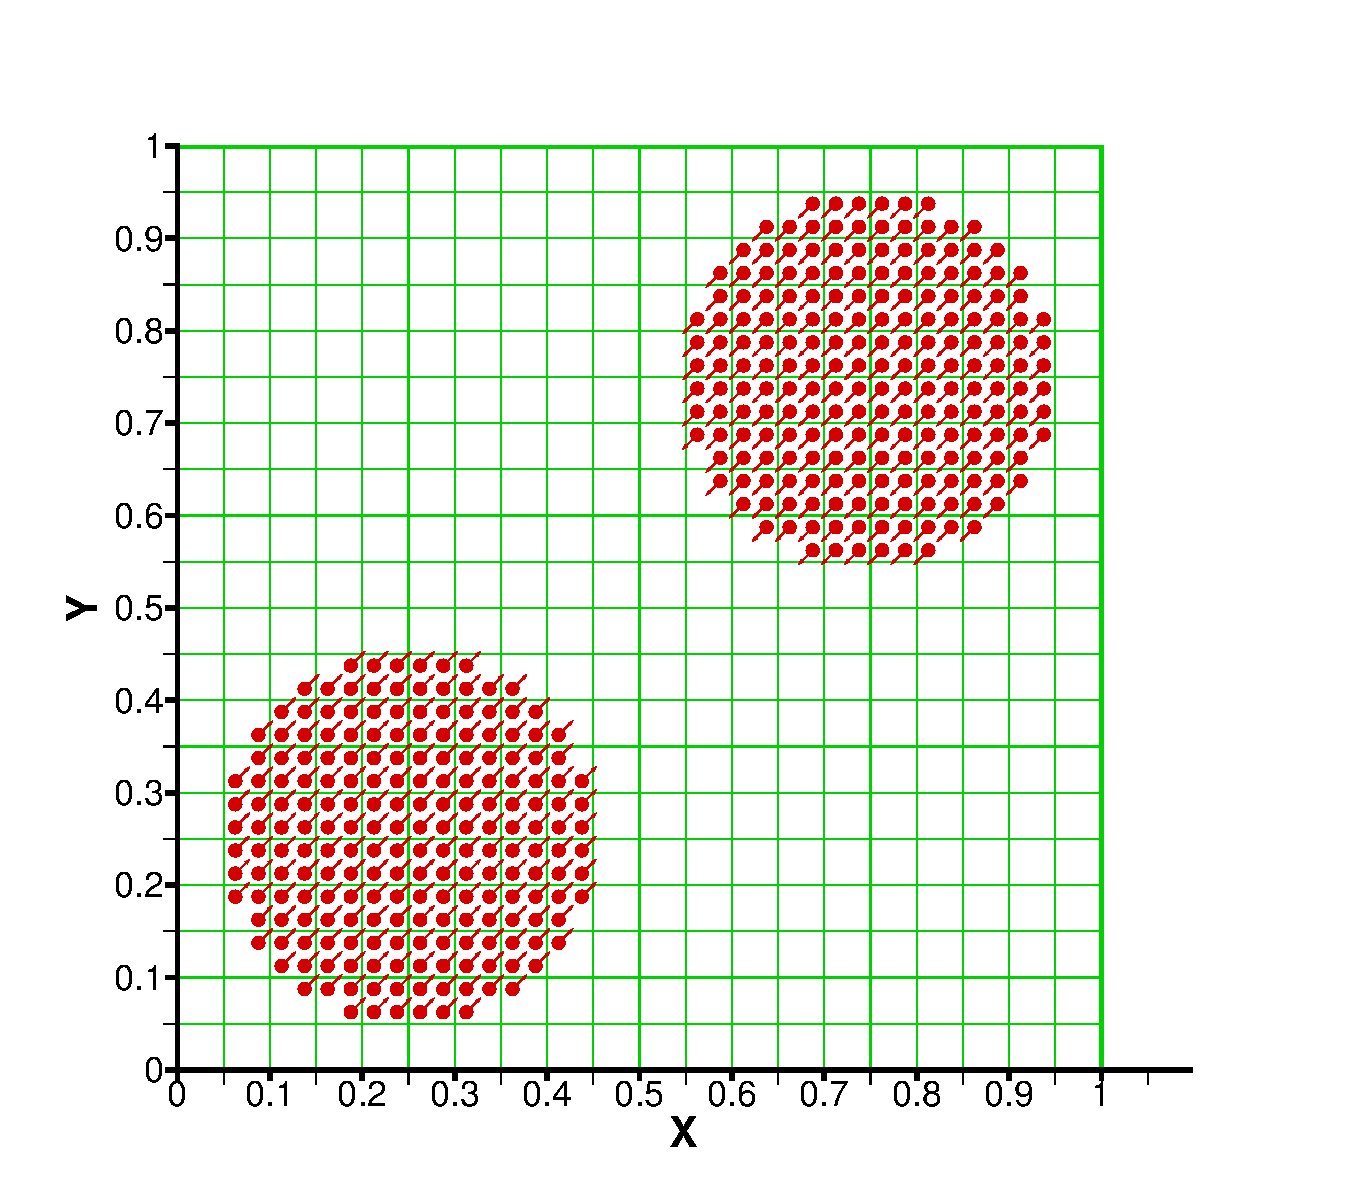
\includegraphics{disks.pdf}}
  \caption{\label{fig-disks_init} Initial particle representation of two
                                colliding disks on an overlying mesh.}
\end{figure}

\section{Vaango Specification} \label{Sec:UintahSpecMPM}
\Vaango input files are constructed in XML format.  Each begins with:
\begin{lstlisting}[language=XML]
<?xml version='1.0' encoding='ISO-8859-1' ?>
\end{lstlisting}
while the remainder of the file is enclosed within the following tags:
\begin{lstlisting}[language=XML]
<Uintah_specification>
</Uintah_specification>
\end{lstlisting}

The following subsections describe the remaining inputs needed to construct
an input file for an MPM simulation.  The order of the various sections 
of the input file is not important.  
\begin{WarningBox}
The MPM, ICE and MPMICE components
are dimensionless calculations.  It is the responsibility of the analyst
to provide the following inputs using a consistent set of units.
\end{WarningBox}

\subsection{Common Inputs} \label{Sec:commonInputs}
Each \Vaango component is invoked using a single executable called
\Textsfc{vaango}, which chooses the type of simulation
to execute based on the \Textsfc{SimulationComponent} tag in the
input file.  For the case of MPM simulations, this looks like:
\begin{lstlisting}[language=XML]
 <SimulationComponent type="mpm" />
\end{lstlisting}

There are a number of fields that are required for any component.  The first
is that describing the timestepping parameters, these are largely common to
all components, and are described in Section~\ref{Sec:TimeRelatedVariables}.
The only one that bears commenting on at this point is:
\begin{lstlisting}[language=XML]
  <timestep_multiplier>    0.5     </timestep_multiplier>
\end{lstlisting}
This is effectively the CFL number for MPM simulations, that is the number
multiplied by the timestep size that is automatically calculated by the MPM
code.  Experience indicates that one should generally keep this value below
$0.5$, and should expect to use smaller values for high-rate, large-deformation
simulations.

The next field common to the input files for all components is:
\begin{lstlisting}[language=XML]
   <DataArchiver>
   </DataArchiver>
\end{lstlisting}
This is described in Section~\ref{Sec:DataArchiver}.  To see a list of
variables available for saving in MPM simulations, execute the following
command from the \Textsfc{StandAlone} directory:

\begin{lstlisting}[backgroundcolor=\color{background}]
inputs/labelNames mpm
\end{lstlisting}
Note that for visualizing particle data, one must save \Textsfc{p.x,}
and at least one other variable by which to color the particles.

The other principle common field is that which describes the computational
grid.  For MPM, this is typically broken up into two parts, the
\Textsfc{Level} section specifies the physical extents and spatial
resolution of the grid.  For more information, consult Section~\ref{Sec:Grid}.
The other part specifies kinematic boundary conditions on the grid boundaries.
These are discussed below in Section~\ref{Sec:MPM_BCs}.

\subsection{Physical Constants} \label{Sec:physicalConstants}
The only physical constant required (or optional for that matter) for
MPM simulations is gravity, this is specified as:

\begin{lstlisting}[language=XML]
<PhysicalConstants>
   <gravity>            [0,0,0]   </gravity>
</PhysicalConstants>
\end{lstlisting}

\subsection{MPM Flags} \label{Sec:MPMFlags}

There are many options available when running MPM simulations.  These
are generally specified in the \Textsfc{MPM} section of the input file.
\begin{NoteBox}
Most options have default values and are not required to be specified
unless the defaults need to be changed.
\end{NoteBox}

Some of these options are described below:
\begin{itemize}
  \item \Textmag{Axisymmetry:}  The \Textsfc{axisymmetric} flag is used
    to indicate that an axisymmetric simulation should be conducted instead
    of the usual three-dimensional simulation.  

    \Textcad{Options:} \Textsfc{true} or \Textsfc{false}\\
    \Textcad{Default:} \Textsfc{false}.

    All axisymmetric simulations
    assume that the plane of rotational symmetry is the $xy$-plane,
    axisymmetric $r$-coordinate coincides with the grid $x$-direction, 
    axisymmetric $z$-coordinate conincides 
    with the grid $y$-direction, and that the axisymmetric $\theta$-coordinate is 
    in the $z$-direction of the grid. The
    \Textsfc{Grid} for axisymetric computations must be only one cell thick
    in the $z$-direction. \Textsfc{Plane strain} calcuations can be simulated
    by applying appropriate grid boundary conditions in 3D.  \Textsfc{Plane stress}
    calculatons are not alowed in \Vaango.
    \begin{lstlisting}[language=XML]
    <MPM>
      <axisymmetric> false </axisymmetric>
    </MPM>
    \end{lstlisting}

  \item \Textmag{Time integrator:}  The \Textsfc{time\_integrator} flag 
    determine the type of integration to be used in the \MPM simulation.

    \Textcad{Options:} \Textsfc{explicit}, \Textsfc{implicit}, or \Textsfc{fracture}.\\
    \Textcad{Default:} \Textsfc{explicit}.

    If the explicit option is chosen integration is done using forward Euler,
    while implicit uses bacward Euler.  if the fracture option is chosen, some
    special integration features needed for \Textsfc{FractureMPM} are activated.

    \begin{lstlisting}[language=XML]
    <MPM>
      <time_integrator> explicit </time_integrator>
    </MPM>
    \end{lstlisting}

  \item \Textmag{Interpolator:}  The \Textsfc{interpolator} flag indicates the
    interpolation technique to be used to interpolate from the grid to particles
    and to project particle data to the grid.

    \Textcad{Options:} \Textsfc{linear}, \Textsfc{gimp}, \Textsfc{3rdorderBS}
                       \Textsfc{4thorderBS}, \Textsfc{cpdi}, or \Textsfc{cpti} \\
    \Textcad{Default:} \Textsfc{linear}.

    The \Textsfc{linear} option activates traditional MPM with linear grid interpolation
    functions.  \Textsfc{gimp} activates the GIMP algorithm. \Textsfc{3rdorderBS} and
    \Textsfc{4thorderBS} activate third- and fourth-order B-spline interpolation.
    \Textsfc{cpdi} and \Textsfc{cpti} activate the CPDI and CPTI interpolators.
    \begin{lstlisting}[language=XML]
    <MPM>
      <interpolator> gimp </interpolator>
    </MPM>
    \end{lstlisting}

    Options other than \Textsfc{linear} require an \Textsfc{extraCells} tag
    (ghost cells) when specifying the \Textsfc{Grid}:
    \begin{lstlisting}[language=XML]
    <Grid>
      ...
      <extraCells> [1,1,1] </extraCells>
    </Grid>
    \end{lstlisting}
    For axisymmetric simulations the $z$-value of \Textsfc{extraCells} can be 0.

    The \Textsfc{CPDI} interpolator may also require a critical length value,
    \Textsfc{cpdi\_lcrit}, 
    that determines the maximum distance a particle can extend before its full
    extent is ignore by the CPDI algorithm.

    \Textcad{Default:} \Textsfc{1.0e10}.
    \begin{lstlisting}[language=XML]
    <MPM>
      <interpolator> cpdi </interpolator>
      <cpdi_lcrit> 1.0e3 </cpdi_lcrit>
    </MPM>
    \end{lstlisting}

  \item \Textmag{Particle color:}  The \Textsfc{with\_color} flag indicates that
    color tags are being used in the simulation.  Each geometry object can 
    then be assigned a \Textsfc{\textless color \textgreater} tag which has 
    an integer vaue.

    \Textcad{Options:} \Textsfc{true} or \Textsfc{false}\\
    \Textcad{Default:} \Textsfc{false}.

    The color flag is particulary useful for debugging simulations where a
    particular material is associated with a large number of geometry objects.
    \begin{lstlisting}[language=XML]
    <MPM>
      <with_color> false </with_color>
    </MPM>
    \end{lstlisting}

  \item \Textmag{Damping:}  Two types of damping are allowed in \Vaango : a
    velocity-based damping that is applied during the integration of the
    accleration, and a Richtmyer-von Neumann artificial viscosity that
    is slightly more complex (see the Theory Manual for details).

    Velocity-based damping is always active and controlled by the
    \Textsfc{artificial\_damping\_coeff} flag.

    \Textcad{Default:} 0.0
    \begin{lstlisting}[language=XML]
    <MPM>
      <artificial_damping_coeff> 0.0 </artificial_damping_coeff>
    </MPM>
    \end{lstlisting}

    Richtmyer-von Neumann viscosity is activated by the \Textsfc{artificial\_viscosity}
    flag and requires two parameters, \Textsfc{artificial\_viscosity\_coeff1} and
    \Textsfc{artificial\_viscosity\_coeff1}.  

    \Textcad{Options:} \Textsfc{true} or \Textsfc{false}\\
    \Textcad{Defaults:} false, 0.2, 2.0
    \begin{lstlisting}[language=XML]
    <MPM>
      <artificial_viscosity> false </artificial_viscosity>
      <artificial_viscosity_coeff1> 0.2 </artificial_viscosity_coeff1>
      <artificial_viscosity_coeff2> 2.0 </artificial_viscosity_coeff2>
    </MPM>
    \end{lstlisting}

    Viscous heating is automatically turned
    on when the \Textsfc{artificial\_viscosity} flag is on.  If \Textsfc{artificial\_viscosity}
    is off, viscous heating can still be activated using the
    \Textsfc{artificial\_viscosity\_heating} tag.  However, this is typically not
    allowed in a simulation.
    
    \Textcad{Options:} \Textsfc{true} or \Textsfc{false}\\
    \Textcad{Default:} false
    \begin{lstlisting}[language=XML]
    <MPM>
      <artificial_viscosity_heating> false </artificial_viscosity_heating>
    </MPM>
    \end{lstlisting}

  \item \Textmag{Deformation gradient:}  Deformation gradient computation algorithms
    can be switched by activating the \Textsfc{deformation\_gradient} tag.  See
    the \Vaango Theory Manual for further information.

    \Textcad{Options:} \Textsfc{first\_order}, \Textsfc{sybcycling}, 
                       \Textsfc{taylor\_series}, or \Textsfc{cayley\_hamilton}\\
    \Textcad{Default:} \Textsfc{first\_order}
    \begin{lstlisting}[language=XML]
    <MPM>
      <deformation_gradient algorithm="taylor_series">
        <num_terms> 5 </num_terms>
      </deformation_gradient>
    </MPM>
    \end{lstlisting}

    A parameter, \Textsfc{num\_terms}, indicating the number of terms of the Taylor 
    series to be evaluated can also be added to the tag.  The default value is 1.
    

  \item \Textmag{Load curves:}
  

  \item \Textmag{Boundary traction faces:}  For some special simulations, we
    may require the contact tractions at the domain boundaries to be
    computed and saved.  This feature is activated using the
    \Textsfc{boundary\_traction\_faces} flag which takes a list of
    text strings as input.  The allowed values of \Textsfc{xminus},

    \Textcad{Options:} \Textsfc{xplus}, \Textsfc{yminus}, \Textsfc{yplus}, \Textsfc{zminus},
    and \Textsfc{zplus}. \\
    \Textcad{Default:} \Textsfc{[]}.
    \begin{lstlisting}[language=XML]
    <MPM>
      <boundary_traction_faces>[xminus,xplus,zminus]</boundary_traction_faces>
    </MPM>
    \end{lstlisting}
\end{itemize}

Below is a list of these options taken from
\Textsfc{inputs/UPS\_SPEC/mpm\_spec.xml} 
This file also gives possible values, or at least expected datatype,
for these flags.  A description of their functionality is forthcoming,
in the meantime, consult the code and input files.  A default value is
set for many, see \Textsfc{MPM/MPMFlags.cc} for more.

\begin{lstlisting}[language=XML]
    <MPM>
     <!-- These are commonly used options -->
      <artificial_damping_coeff           spec="OPTIONAL DOUBLE 'positive'"/>
      <artificial_viscosity               spec="OPTIONAL BOOLEAN" />
      <artificial_viscosity_coeff1        spec="OPTIONAL DOUBLE" />
      <artificial_viscosity_coeff2        spec="OPTIONAL DOUBLE" />
      <axisymmetric                       spec="OPTIONAL BOOLEAN" />
      <boundary_traction_faces            spec="OPTIONAL STRING" />
      <DoExplicitHeatConduction           spec="OPTIONAL BOOLEAN" />
      <DoPressureStabilization            spec="OPTIONAL BOOLEAN" />
      <erosion                            spec="OPTIONAL NO_DATA"
            attribute1="algorithm REQUIRED STRING 'none, KeepStress, ZeroStress, RemoveMass'" />
      <interpolator                       spec="OPTIONAL STRING 'linear, gimp, 3rdorderBS, 4thorderBS'" />
      <minimum_particle_mass              spec="OPTIONAL DOUBLE 'positive'"/>
      <minimum_mass_for_acc               spec="OPTIONAL DOUBLE 'positive'"/>
      <maximum_particle_velocity          spec="OPTIONAL DOUBLE 'positive'"/>
      <testForNegTemps_mpm                spec="OPTIONAL BOOLEAN" />
      <time_integrator                    spec="OPTIONAL STRING 'explicit, fracture, implicit'" />
      <use_load_curves                    spec="OPTIONAL BOOLEAN" />
      <UsePrescribedDeformation           spec="OPTIONAL BOOLEAN" />
      <withColor                          spec="OPTIONAL BOOLEAN" />

     <!-- These are not commonly used options -->
      <CanAddMPMMaterial                  spec="OPTIONAL BOOLEAN" />
      <create_new_particles               spec="OPTIONAL BOOLEAN" />
      <do_contact_friction_heating        spec="OPTIONAL BOOLEAN" />
      <do_grid_reset                      spec="OPTIONAL BOOLEAN" />
      <DoThermalExpansion                 spec="OPTIONAL BOOLEAN" />
      <ForceBC_force_increment_factor     spec="OPTIONAL DOUBLE" />
      <manual_new_material                spec="OPTIONAL BOOLEAN" />
      <interpolateParticleTempToGridEveryStep spec="OPTIONAL BOOLEAN" />
      <temperature_solve                  spec="OPTIONAL BOOLEAN" />

     <!-- THE FOLLOWING APPLY ONLY TO THE IMPLICIT MPM CODE -->
      <dynamic                            spec="OPTIONAL BOOLEAN" />
      <solver                             spec="OPTIONAL STRING 'petsc, simple'" />
      <convergence_criteria_disp          spec="OPTIONAL DOUBLE 'positive'"/>
      <convergence_criteria_energy        spec="OPTIONAL DOUBLE 'positive'"/>
      <num_iters_to_decrease_delT         spec="OPTIONAL INTEGER" />
      <num_iters_to_increase_delT         spec="OPTIONAL INTEGER" />
      <iters_before_timestep_restart      spec="OPTIONAL INTEGER" />
      <DoTransientImplicitHeatConduction  spec="OPTIONAL BOOLEAN" />
      <delT_decrease_factor               spec="OPTIONAL DOUBLE" />
      <delT_increase_factor               spec="OPTIONAL DOUBLE" />
      <DoImplicitHeatConduction           spec="OPTIONAL BOOLEAN" />
      <DoMechanics                        spec="OPTIONAL BOOLEAN" />

      <!-- THE FOLLOWING APPLY ONLY TO THE FRACTURE MPM CODE -->
      <dadx                               spec="OPTIONAL DOUBLE" />
      <smooth_crack_front                 spec="OPTIONAL BOOLEAN" />
      <calculate_fracture_parameters      spec="OPTIONAL BOOLEAN" />
      <do_crack_propagation               spec="OPTIONAL BOOLEAN" />
      <use_volume_integral                spec="OPTIONAL BOOLEAN" />
    </MPM>
\end{lstlisting}



\subsection{Material Properties} \label{Sec:mat_props}

The \Textsfc{Material Properties} section of the input file
actually contains not only those, but also the geometry and initial
condition data as well.  Below is a simple example, copied from
\Textsfc{inputs/MPM/disks.ups.}  The \Textsfc{name} field
is optional.  The first field is the material \Textsfc{density}.
The \Textsfc{constitutive\_model} field refers
to the model used to generate a stress tensor on each material point.
The use of these models is described in detail in
Section~\ref{Sec:ConstitutiveModels}.  Next are the thermal transport properties,
\Textsfc{thermal\_conductivity} and 
\Textsfc{specific\_heat}.  Note that these are required even if
heat conduction is not being computed.  These are the required material
properties.  There are additional optional parameters that are used in
other auxiliary calculations, for a list of these
see the \Textsfc{inputs/UPS\_SPEC/mpm\_spec.xml}.

Next is the specification of the geometry, and, along with it, the initial
state of the material contained in that geometry.  For more information on
how initial geometry can be specified, see Section~\ref{Sec:GeometryObjects}.  Within the
\Textsfc{geom\_object} is the \Textsfc{res} field.  This
indicates how many particles per cell are to be used in each of the 
coordinate directions.  Following that are initial values for velocity and
temperature.  Finally, the \Textsfc{color} designation has a number
of uses, for example when one wishes to identify initially distinct regions
of the same material.  In Section~\ref{Sec:OTFA_MPM} is a description of how
this field is used to identify particles for on the fly data extraction.

An arbitray number of \Textsfc{material} fields can be specified.
As the calculation proceeds, each of these materials has their own field
variables, and, as such, each material behaves independently of the others.
Interactions between materials occur as a result of ``contact" models.
Their use is described in detail in Section~\ref{Sec:Contact}.

\begin{lstlisting}[language=XML]
    <MaterialProperties>
       <MPM>
           <material name="disks">
              <density>1000.0</density>
              <constitutive_model type="comp_mooney_rivlin">
                 <he_constant_1>100000.0</he_constant_1>
                 <he_constant_2>20000.0</he_constant_2>
                 <he_PR>.49</he_PR>
              </constitutive_model>
              <thermal_conductivity>1.0</thermal_conductivity>
              <specific_heat>5</specific_heat>
              <geom_object>
                  <cylinder label = "gp1">
                     <bottom>[.25,.25,.05]</bottom>
                     <top>[.25,.25,.1]</top>
                     <radius> .2 </radius>
                  </cylinder>
                  <res>[2,2,2]</res>
                  <velocity>[2.0,2.0,0]</velocity>
                  <temperature>300</temperature>
                  <color>             0               </color>
               </geom_object>
           </material>

           <contact>
             <type>null</type>
             <materials>[0]</materials>
           </contact>
       </MPM>
    </MaterialProperties>
\end{lstlisting}

\subsection{Contact}  \label{Sec:Contact}
When multiple materials are specified in the input file, each material
interacts with its own field variables.  In other words, each material has
its own mass, velocity, acceleration, etc.  Without any mechanism for their
interaction, each material would behave as if it were the only one in the
domain.  Contact models provide the mechanism by which to specify rules
for inter material interactions.  There are a number of contact models
from which to choose, the use of each is described next.  See the input
file segment in Section~\ref{Sec:mat_props} for an example of their proper
placement in the input file, namely, after all of the MPM materials have
been described.

\subsubsection{Null contact}
The simplest contact model is the \Textsfc{null} model, which indicates
that no inter material interactions are to take place.  This is typically only
used in single material simulations.  Its usage looks like:

\begin{lstlisting}[language=XML]
           <contact>
             <type>null</type>
           </contact>
\end{lstlisting}

\subsubsection{Single velocity contact}
The next simplest model is the \Textsfc{single\_velocity} model.
The basic MPM formulation provides ``free" no-slip, no-interpenetration
contact, assuming that all particle data communicates with a single field
on the grid.  For a single material simulation with multiple objects, that
is the case.  If one wishes to achieve that behavior in \Vaango-MPM when
multiple materials are present, the \Textsfc{single\_velocity} contact
model should be used.  It is specified as:

\begin{lstlisting}[language=XML]
           <contact>
             <type>single_velocity</type>
             <materials>[0,1]</materials>
           </contact>
\end{lstlisting}
Note that for this, and all of the contact models,
the \Textsfc{materials} tag is optional.  If it is omitted,
the assumption is that all materials will interact via the same contact model.
(This will be further discussed below.)

\subsubsection{Friction contact}
The ultimate in contact models is the \Textsfc{friction} contact 
model.  For a full description, the reader is directed to the paper by
Bardenhagen et al.\cite{Bard2001}.  Briefly, the model both overcomes
some deficiences in the single velocity field contact (either the ``free"
contact or the model described above, which behave identically), and it
enables some additional features.  With single velocity field contact,
initially adjacent objects are treated as if they are effectively stuck
together.  The friction contact model overcomes this by detecting if
materials are approaching or departing at a given node.  If they are
approaching, contact is ``enforced" and if they are departing, another
check is made to determine if the objects are in compression or tension.
If they are in compression, then they are still rebounding from each other,
and so contact is enforced.  If tension is detected, they are allowed
to move apart independently.  Frictional sliding is allowed, based on
the value specified for \Textsfc{mu} and the normal force between
the objects.  An example of the use of this model is given here:

\begin{lstlisting}[language=XML]
           <contact>
              <type>friction</type>
              <materials>[0,1,2]</materials>
              <mu> 0.5 </mu>
           </contact>
\end{lstlisting}

A slightly improved implementation of the Bardenhagen contact model can be
accessed with the alternative tag:
\begin{lstlisting}[language=XML]
           <contact>
              <type>friction_bard</type>
              <materials>[0,1,2]</materials>
              <mu> 0.5 </mu>
           </contact>
\end{lstlisting}

A more recent friction contact algorithm~\cite{Nairn2020}  uses \Textsfc{logistic 
regression} to identify the interface between two (or more) materials in contact.
This model can be activated using:
\begin{lstlisting}[language=XML]
           <contact>
              <type>friction_LR</type>
              <materials>[0,1,2]</materials>
              <mu> 0.5 </mu>
           </contact>
\end{lstlisting}
For more detail, please see the section on \Textsfc{Logistic regression friction contact}
in the theory manual.
\begin{WarningBox}
The logistic regression friction contact model is {\Red not} activated if there is \Textsfc{only
one material} but \Textsfc{multiple geometry objects} in the input file.  Please associate
objects that you would like to interact via friction contact with separate materials.
\end{WarningBox}

\subsubsection{Approach contact}
A slightly simplified version of the friction model is the
\Textsfc{approach} model.  It is the same as the frictional model
above, except that it doesn't make the additional check on the traction
between two bodies at each node.  At times, it is necessary to neglect this,
but some loss of energy will result.  Specification is of the model is 
also nearly identical:

\begin{lstlisting}[language=XML]
           <contact>
              <type>approach</type>
              <materials>[0,1,2]</materials>
              <mu> 0.5 </mu>
           </contact>
\end{lstlisting}

\subsubsection{Specified/Rigid contact}
Finally, the contact infrastructure is also used to provide a moving
displacement boundary condition.  Imagine a billet being smashed by a
rigid platen, for example.  Usage of this model, known as
\Textsfc{specified} contact, looks like:

\begin{lstlisting}[language=XML]
           <contact>
             <type>specified</type>
             <filename>TXC.txt</filename>
             <materials>[0,1,2]</materials>
             <master_material>0</master_material>
             <direction>[1,1,1]</direction>
             <stop_time>1.0 </stop_time>
             <velocity_after_stop>[0, 0, 0]</velocity_after_stop>
           </contact>
\end{lstlisting}
For reasons of backwards compatibility, the
\Textsfc{specified} contact type is interchangable with
\Textsfc{rigid.}  By default, when either model is
chosen, material 0 is the ``rigid" material, although this can be
overridden by the use of the
\Textsfc{master\_material} field.  If no
\Textsfc{filename} field is specified, then the particles of the
rigid material proceed with the velocity that they were given as their
initial condition, either until the reach a computational boundary, or
until the simulation time has reached \Textsfc{stop\_time,} after
which, their velocity becomes that given in the
\Textsfc{velocity\_after\_stop} field.  The \Textsfc{direction}
field indicates in which cartesian directions contact should be specified.
Values of $1$ indicate that contact should be specified, $0$ indicates that
the subject materials should be allowed to slide in that direction.  

If a \Textsfc{filename} field \Textsfc{is} specified, then the user can
create a text file which contains four entries per line.  These are:
\begin{lstlisting}[backgroundcolor=\color{background}]
time1 velocity_x1 velocity_y1 velocity_z1
time2 velocity_x2 velocity_y2 velocity_z2
     .
     .
     .
\end{lstlisting}
The velocity of the rigid material particles will be set to these values,
based on linear interpolation between times, until \Textsfc{stop\_time}
is reached.  

The figures below show how the specified contact algorithm can be used to 
simulate uniaxial tension and compression tests.  The green block is the
rigid master material that moves with a specified velocity.

\begin{minipage}[t]{0.25\textwidth}
  \centering
  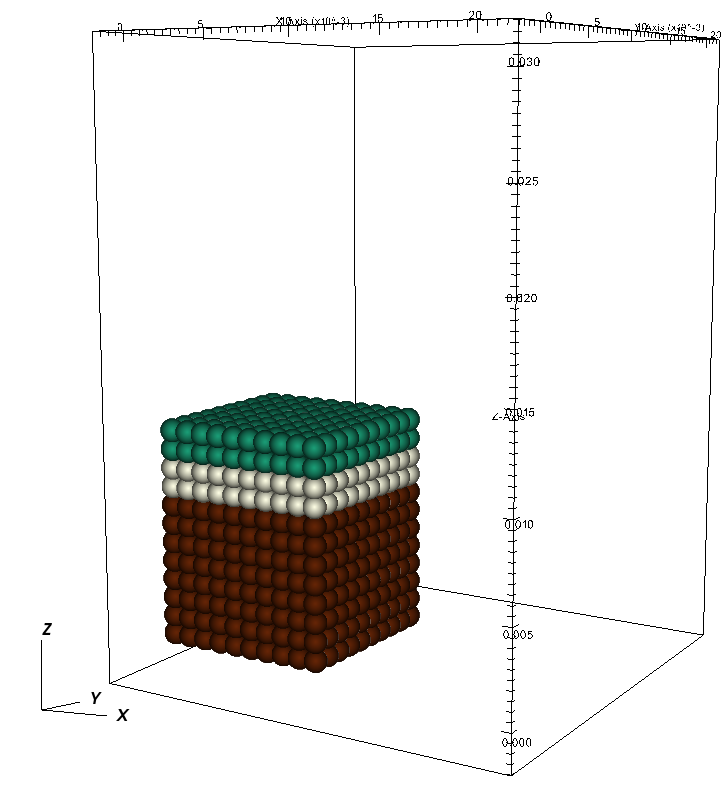
\includegraphics[width=0.9\columnwidth]{FIGS/contact/rigid_tension.png} \\
  {Initial state for tension test.}
\end{minipage}
\begin{minipage}[t]{0.25\textwidth}
  \centering
  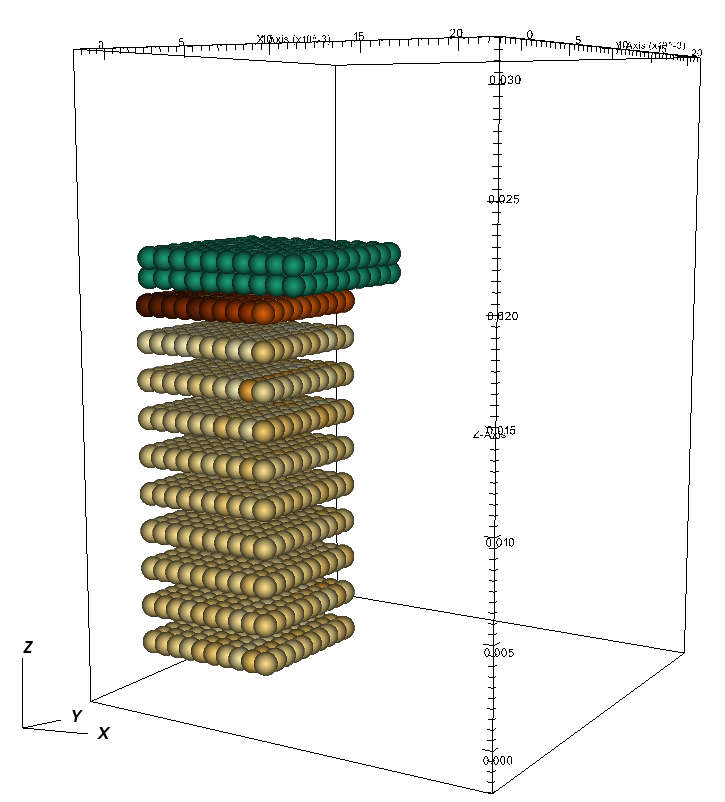
\includegraphics[width=0.9\columnwidth]{FIGS/contact/rigid_tension_end.png}\\
  {Deformed state for tension test.}
\end{minipage}
\begin{minipage}[t]{0.25\textwidth}
  \centering
  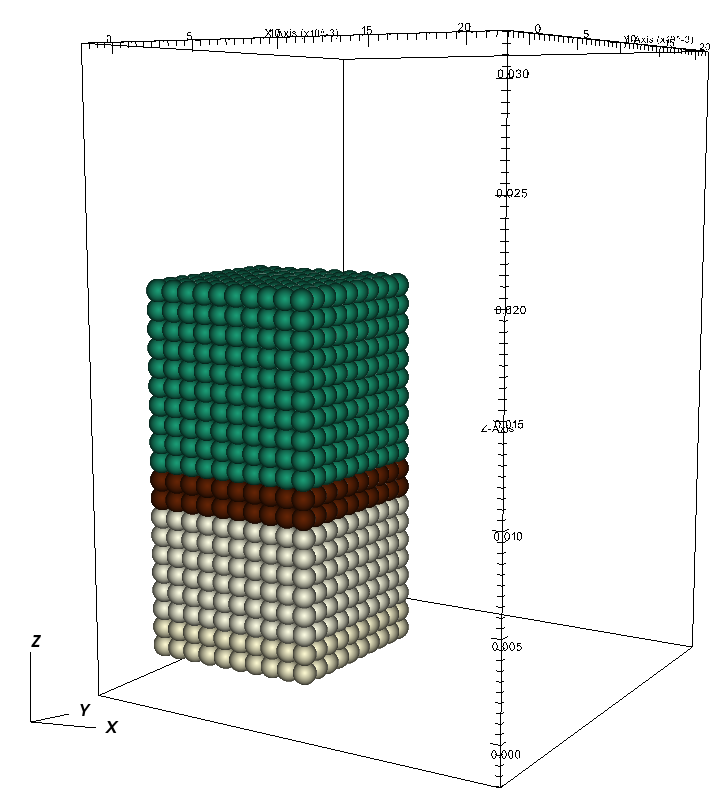
\includegraphics[width=0.9\columnwidth]{FIGS/contact/rigid_compression.png}
  {Initial state for compression test.}
\end{minipage}
\begin{minipage}[t]{0.25\textwidth}
  \centering
  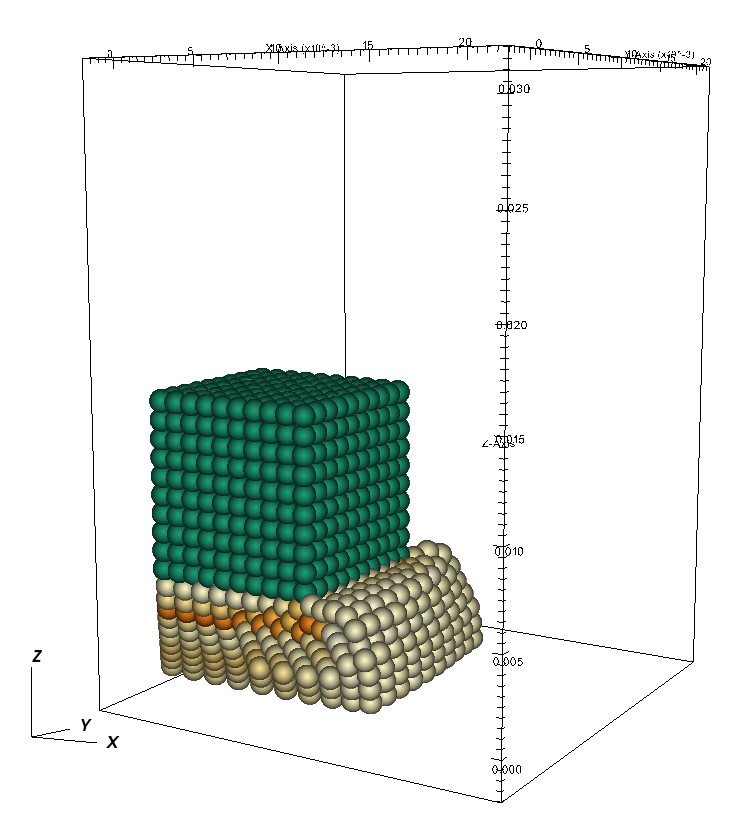
\includegraphics[width=0.9\columnwidth]{FIGS/contact/rigid_compression_end.png}
  {Deformed state for compression test.}
\end{minipage}

An alternative way of performing this type of contact is via surface normals.
In that case, the input has the form:
\begin{lstlisting}[language=XML]
 <contact>
   <type>specified</type>
   <master_material> 0 </master_material>
   <master_material_is_rigid> true </master_material_is_rigid>
   <normal_only> true </normal_only>
 </contact>
\end{lstlisting}
This allows specified contact with arbitrarily moving geometries. In the
figures below, note the motion of the rigid disk to the left and compare it 
to that of the the deformable disk which shows stress waves.  The
motion of the rigid disk is unaffected by the contact event.

\begin{minipage}[t]{0.3\textwidth}
  \centering
  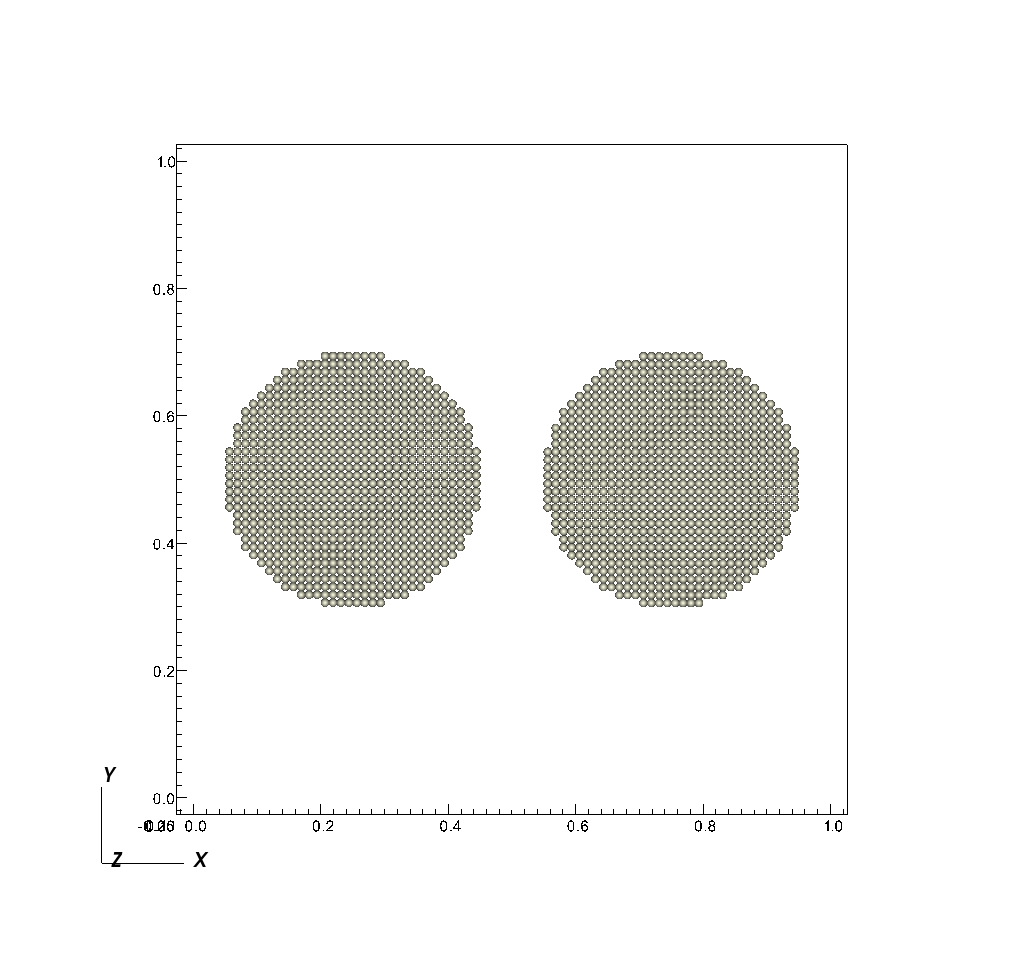
\includegraphics[width=0.9\columnwidth]{FIGS/contact/specified0.png}
\end{minipage}
\begin{minipage}[t]{0.3\textwidth}
  \centering
  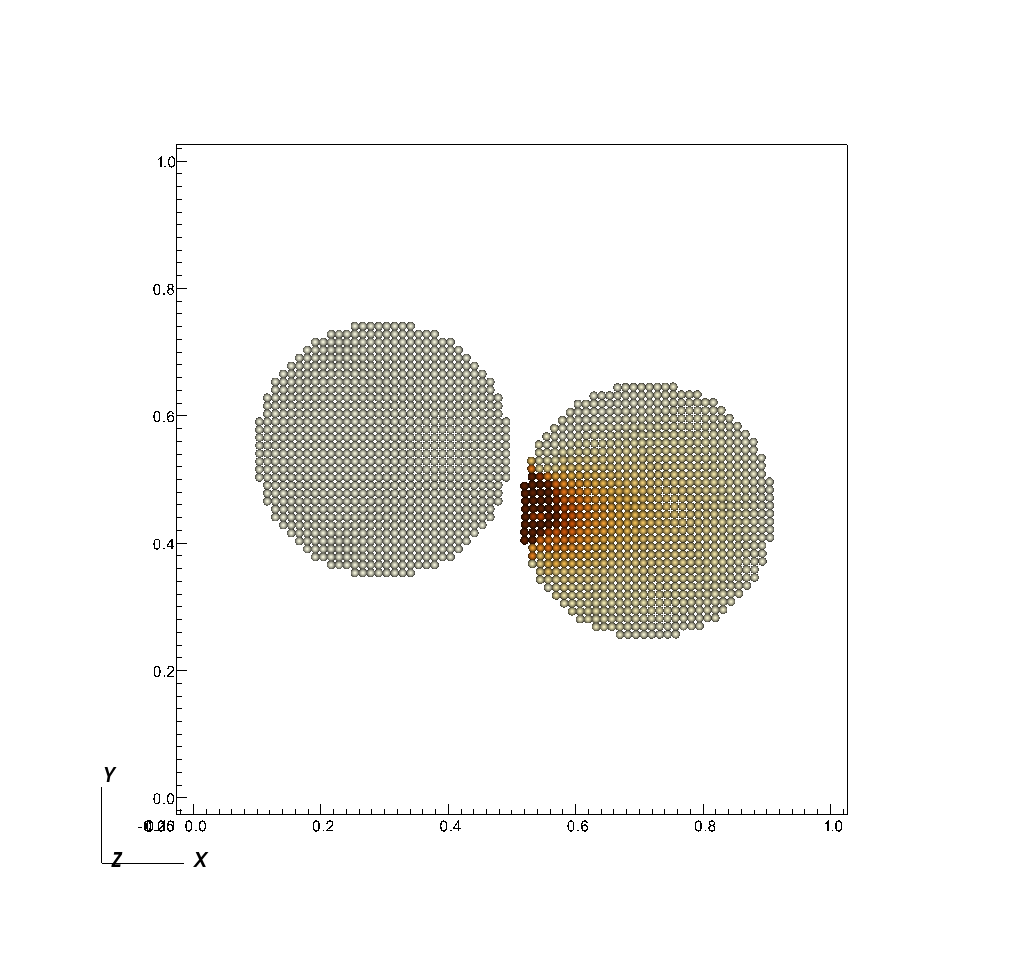
\includegraphics[width=0.9\columnwidth]{FIGS/contact/specified1.png}
\end{minipage}
\begin{minipage}[t]{0.3\textwidth}
  \centering
  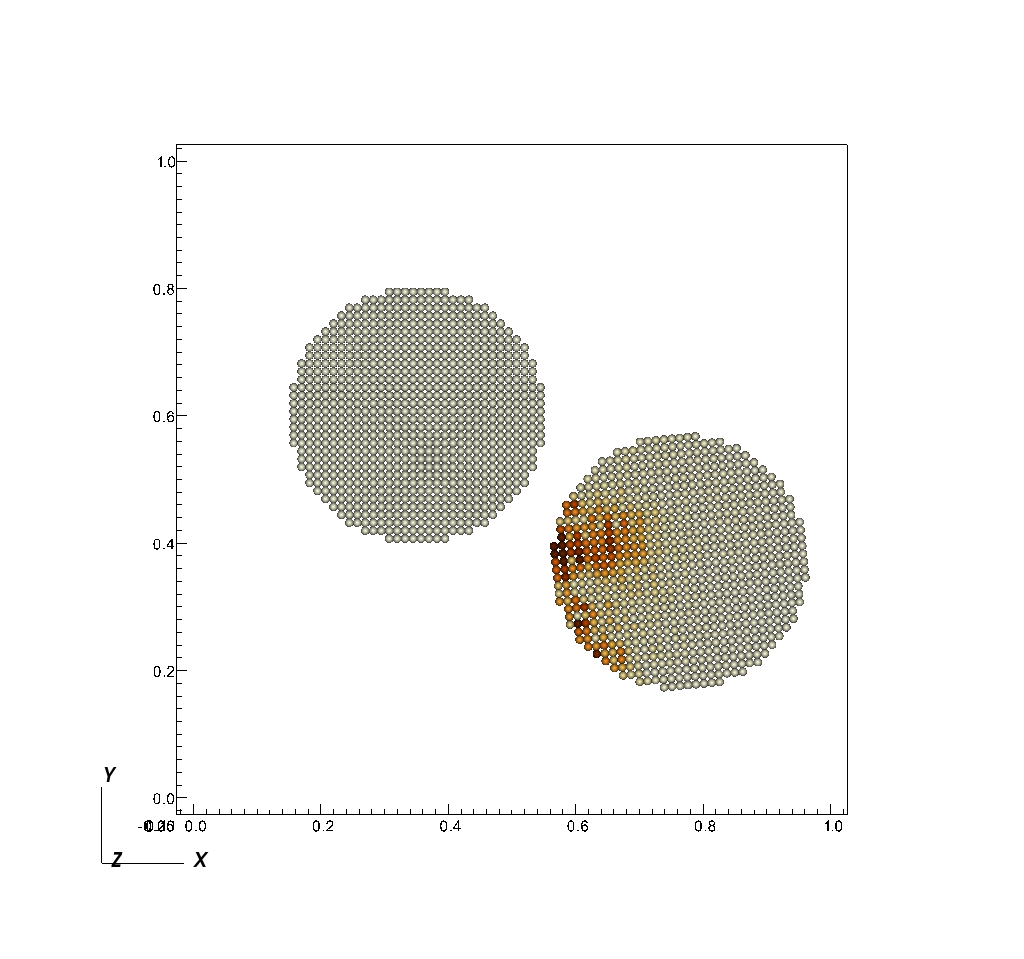
\includegraphics[width=0.9\columnwidth]{FIGS/contact/specified2.png}
\end{minipage}

\begin{minipage}[t]{0.3\textwidth}
  \centering
  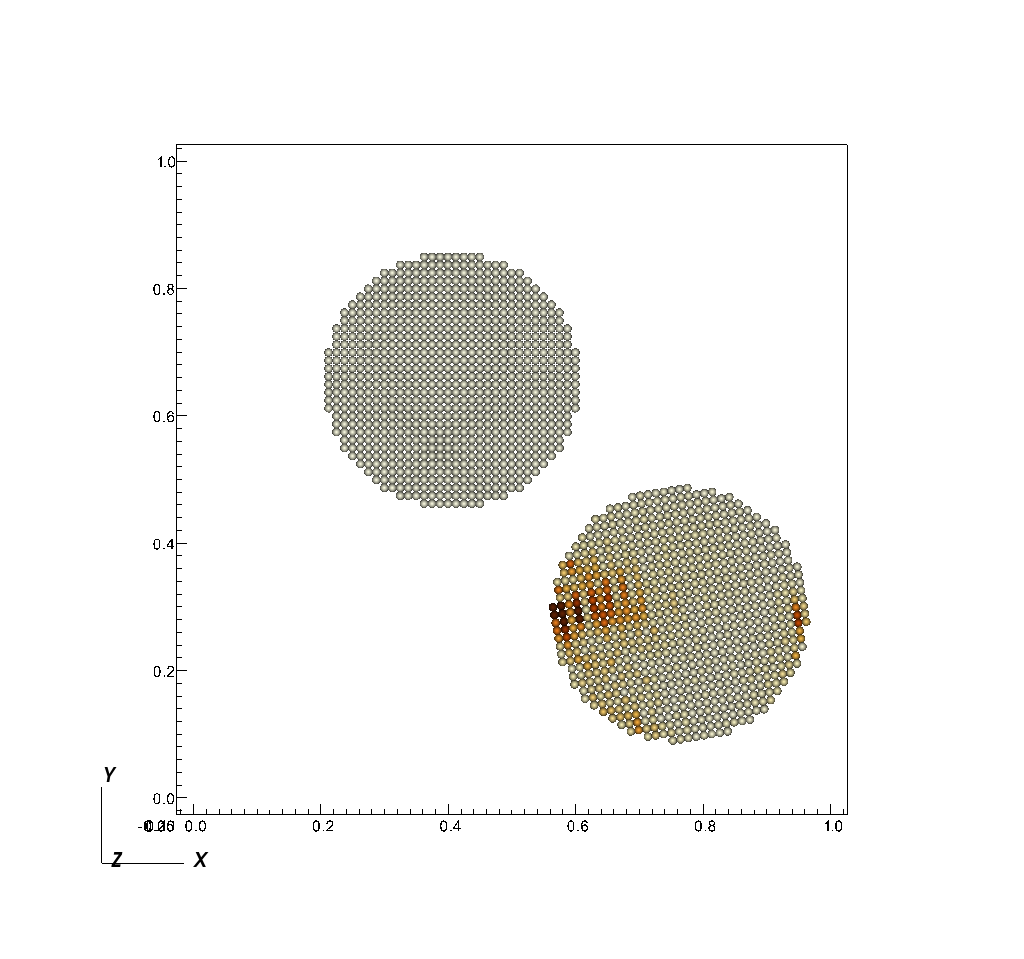
\includegraphics[width=0.9\columnwidth]{FIGS/contact/specified3.png}
\end{minipage}
\begin{minipage}[t]{0.3\textwidth}
  \centering
  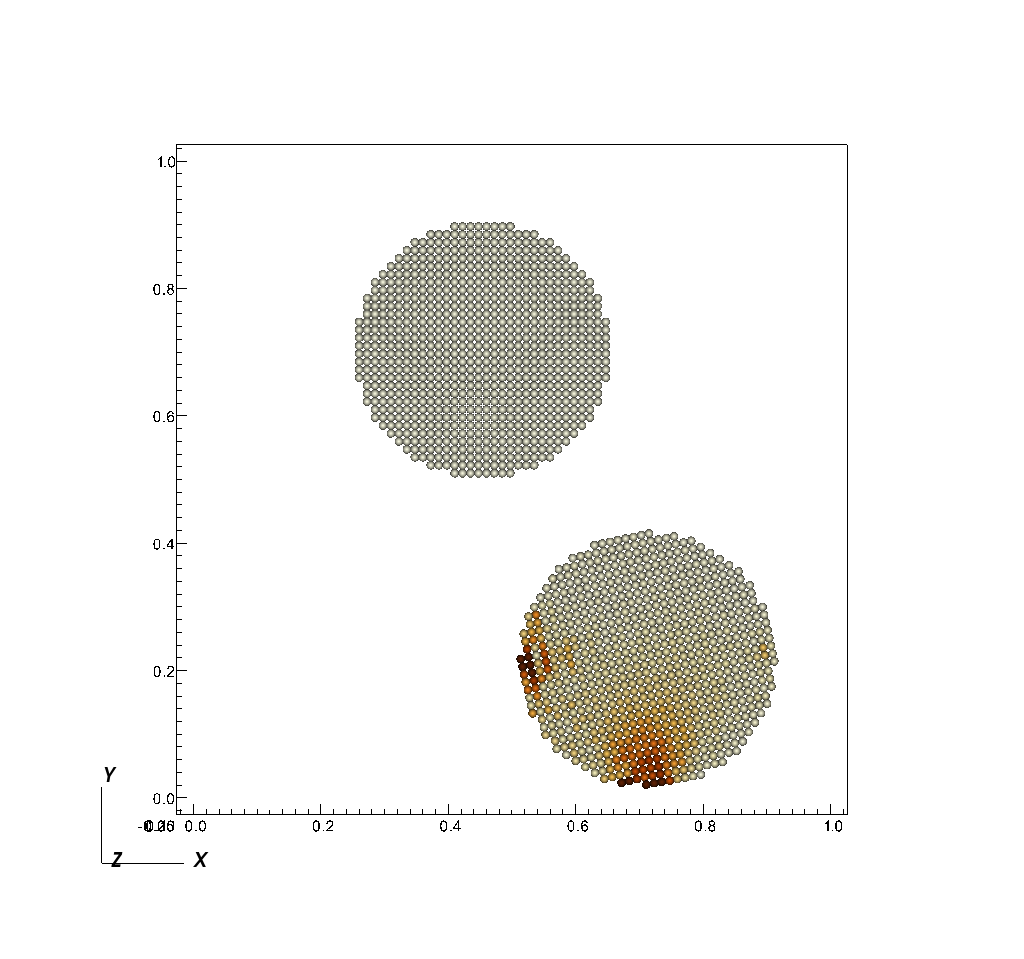
\includegraphics[width=0.9\columnwidth]{FIGS/contact/specified4.png}
\end{minipage}

\begin{WarningBox}
Note, one should not try to apply traction boundary conditions
(via the  \Textsfc{PhysicalBC} tag), to the rigid material used in this type of 
contact, as this constitutes trying to mix displacement and traction boundary
conditions. 
\end{WarningBox}

\subsubsection{Composite contact}
Finally, it is possible to specify more than one contact model.  Suppose
one has a simulation with three materials, one rigid, and the other two
deformable.  The user may want to have the rigid material interact in a
rigid manner with the other two materials, while the two deformable materials
interact with each other in a single velocity field manner.  Specification
for this, assuming the rigid material is $0$ would look like:

\begin{lstlisting}[language=XML]
            <contact>
                <type>single_velocity</type>
                <materials>[1,2]</materials>
            </contact>

            <contact>
                <type>specified</type>
                <filename>prof.txt</filename>
                <stop_time>1.0</stop_time>
                <direction>[0, 0, 1]</direction>
            </contact>
\end{lstlisting}
An example of this usage can be found in \Textsfc{inputs/MPM/twoblock-single-rigid.ups.}




\section{BoundaryConditions} \label{Sec:MPM_BCs}

Boundary conditions must be specified on each face of the computational
domain $(x^-, x^+, y^-, y^+,z^-,z^+)$ for each material.  An example of their
specification is as follows, where the entire \Textsfc{Grid} field
is included for context:
\begin{lstlisting}[language=XML]
    <Grid>
       <BoundaryConditions>
         <Face side = "x-">
             <BCType id = "all" var = "Dirichlet" label = "Velocity">
                   <value> [0.0,0.0,0.0] </value>
             </BCType>
         </Face>
         <Face side = "x+">
            <BCType id = "all" var = "Neumann" label = "Velocity">
                 <value> [0.0,0.0,0.0] </value>
            </BCType>
         </Face>
         <Face side = "y-">
           <BCType id = "all" var = "Dirichlet" label = "Velocity">
                  <value> [0.0,0.0,0.0] </value>
           </BCType>
         </Face>
         <Face side = "y+">
           <BCType id = "all" var = "Neumann" label = "Velocity">
                  <value> [0.0,0.0,0.0] </value>
           </BCType>
         </Face>
         <Face side = "z-">
           <BCType id = "all" var = "symmetry" label = "Symmetric"> </BCType>
         </Face>
         <Face side = "z+">
           <BCType id = "all" var = "symmetry" label = "Symmetric"> </BCType>
         </Face>
       </BoundaryConditions>
       <Level>
\end{lstlisting}

... See Section~\ref{Sec:Grid} ...

\begin{lstlisting}[language=XML]
       </Level>
    </Grid>
\end{lstlisting}

The three main types of numerical boundary conditions (BCs) that can
be applied are ``Neumann", ``Dirichlet", and ``Symmetric", and the use of
each is illustrated above.  In the case of
MPM simulations, Neumann BCs are used when one wishes to allow particles to
advect freely out of the computational domain.  Dirichlet BCs are used to
specify a velocity, zero or otherwise (indicated by the \Textsfc{value}
tag), on one of the computational boundaries.
Symmetric BCs are used to indicate a plane of symmetry.  This has a variety
of uses.  The most obvious is simply when a simulation of interest has symmetry
that one can take advantage of to reduce the cost of a calculation.  Similarly,
since \Vaango is a three-dimensional code, if one wishes to achieve plane-strain
conditions, this can be done by carrying out a simulation that is one cell thick
with Symmetric BCs applied to each face of the plane, as in the example above.
Finally, Symmetric BCs also provide a free slip boundary.

There is also the field \Textsfc{id = "all"}.  In principal, one could
set different boundary condition types for different materials.  In practice,
this is rarely used, so the usage illustrated here should be used.

\subsection{Physical Boundary Conditions} \label{sec:PhysicalBCs}

It is often more convenient to apply a specified load at the MPM particles.
The load may be a function of time.  Such a load versus time curve is called
a {\bf load curve}.
In \Vaango, the load curve infrastructure is available for general use
(and not only for particles).  However, it has been implemented only for
a special case of pressure loading.  Namely, a surface is
specified through the use of the \Textsfc{geom\_object} description,
and a pressure vs. time curve is described by specifying their values
at discrete points in time, between which linear interpolation is used
to find values at any time.  At $t=0$, those particles in the vicinity
of the the surface are tagged with a load curve ID, and those particles
are assigned external forces such that the desired pressure is achieved.

We invoke the load curve in the \Textsfc{MPM} section
(See Section~\ref{Sec:MPMFlags}) of the input file
by setting \Textsfc{use\_load\_curves} to \Textbfc{true}.  The default value
is \Textbfc{false}.

In \Vaango, a load curve infrastructure is implemented in the file \\
\Textsfc{.../MPM/PhysicalBC/LoadCurve.h}.  This file is essentially a templated
structure that has the following private data
\begin{lstlisting}[language=Cpp]
  // Load curve information 
  std::vector<double> d_time;
  std::vector<T> d_load;
  int d_id;
\end{lstlisting}
The variable \Textsfc{d\_id} is the load curve ID, \Textsfc{d\_time} is the time,
and \Textsfc{d\_load} is the load.  Note that the load can have any form - scalar,
vector, matrix, etc.

In our current implementation, the actual specification of the load curve
information is in the \Textsfc{PhysicalBC} section of the input file.  The
implementation is limited in that it applies only to pressure boundary
conditions for some special geometries (the implementation is in
\Textsfc{.../MPM/PhysicalBC/PressureBC.cc}).  However, the load curve template can
be used in other, more general, contexts.

A sample input file specification of a pressure load curve is shown below.
In this case, a pressure is applied to the inside and outside of a cylinder.
The pressure is ramped up from 0 to 1 GPa on the inside and from 0 to 0.1 MPa
on the outside over a time of 10 microsecs.
\begin{lstlisting}[language=XML]
   <PhysicalBC>
     <MPM>
       <pressure>
         <geom_object>
           <cylinder label = "inner cylinder">
             <bottom>           [0.0,0.0,0.0]   </bottom>
             <top>              [0.0,0.0,.02]   </top>
             <radius>           0.5             </radius>
           </cylinder>
         </geom_object>
         <load_curve>
           <id>1</id>
           <time_point>
             <time> 0 </time>
             <load> 0 </load>
           </time_point>
           <time_point>
             <time> 1.0e-5 </time>
             <load> 1.0e9 </load>
           </time_point>
         </load_curve>
       </pressure>
       <pressure>
         <geom_object>
           <cylinder label = "outer cylinder">
             <bottom>           [0.0,0.0,0.0]   </bottom>
             <top>              [0.0,0.0,.02]   </top>
             <radius>           1.0             </radius>
           </cylinder>
         </geom_object>
         <load_curve>
           <id>2</id>
           <time_point>
             <time> 0 </time>
             <load> 0 </load>
           </time_point>
           <time_point>
             <time> 1.0e-5 </time>
             <load> 101325.0 </load>
           </time_point>
         </load_curve>
       </pressure>
     </MPM>
   </PhysicalBC>
\end{lstlisting}
The complete input file can be found in \Textsfc{inputs/MPM/thickCylinderMPM.ups}. 
An additional example which is used to achieve triaxial loading can be found
at \Textsfc{inputs/MPM/TXC.ups}.  There, the material geometry is a block, and so
the regions described are flat surfaces upon which the pressure is applied.

\section{On the Fly DataAnalysis} \label{Sec:OTFA_MPM}

In the event that one wishes to monitor the data for a small region of a
simulation at a rate that is more frequent than the what the DataArchiver
can reasonably provide (for reasons of data storage and effect on run time),
\Vaango provides a \Textsfc{DataAnalysis} feature.  As it applies
to MPM, it allows one to specify a group of particles, by assigning those
particles a particular value of the \Textsfc{color} parameter.
In addition, a list of variables and a frequency of output is provided.
Then, at run time, a sub-directory (\Textsfc{particleExtract/L-0})
is created inside the uda which contains
a series of files, named according to their particle IDs, one for each
tagged particle.  Each of these files contains the time and position for
that particle, along with whatever other data is specified.  {\bf To use this
feature, one must include the} \Textsfc{withColor>   true   </withColor}
{\bf tag in the} \Textsfc{MPM} {\bf section of the input file.}
(See Section~\ref{Sec:MPMFlags}.)

The following input file snippet is taken from
\Textsfc{inputs/MPM/disks.ups}  
\begin{lstlisting}[language=XML]
    <DataAnalysis>
       <Module name="particleExtract">

        <material>disks</material>
        <samplingFrequency> 1e10 </samplingFrequency>
        <timeStart>          0   </timeStart>
        <timeStop>          100  </timeStop>
        <colorThreshold>
          0
        </colorThreshold>

        <Variables>
          <analyze label="p.velocity"/>
          <analyze label="p.stress"/>
        </Variables>

      </Module>
    </DataAnalysis>
\end{lstlisting}

For all particles that are assigned a color greater than the
\Textsfc{colorThreshold>,} the variables
\Textsfc{p.velocity} and
\Textsfc{p.stress} are saved every every
$1/$\Textsfc{samplingFrequency} time units, starting at
\Textsfc{timeStart} until
\Textsfc{timeStop>.}

It is also possible to save grid based data with this module,
see Section~\ref{Sec:ICE} for more information.

\section{Prescribed Motion} \label{Sec:PrescribedMotion} The prescribed motion
capability in \Vaango allows the user to prescribe arbitrary material
deformations and superimposed rotations.  This capability is particularly
useful in verifying that the constitutive model is behaving as expected and is
frame indifferent.  To prescribe material motion the following tag must be
included in the \Textsfc{MPM} section of the input file:

\begin{lstlisting}[language=XML]
 <MPM>
     <UsePrescribedDeformation>true</UsePrescribedDeformation>
 </MPM>
\end{lstlisting}

The desired motion must then be specified in a file named \Textsfc{time\_defgrad\_rotation}.  The format of this file is as follows:

\begin{lstlisting}[backgroundcolor=\color{background}]
t0 F11 F12 F13 F21 F22 F23 F31 F32 F33 theta0 a0 a1 a2
t1 F11 F12 F13 F21 F22 F23 F31 F32 F33 theta1 a0 a1 a2
. . .
tn F11 F12 F13 F21 F22 F23 F31 F32 F33 thetan a0 a1 a2

\end{lstlisting}
where the first column is time, columns two through ten are the nine components of the prescribed deformation gradient, the eleventh column is the desired rotation angle, and the remaining three columns are the three components of the axis of prescribed rotation.  The components of the deformation gradient are linearly interpolated for times between those specified in the table.  The axis of rotation may be changed for each specified time.  As a result, the angle of rotation about the specified axis linearly increases from zero to the specified value at the end of the specified interval.  For example, the following table:

\begin{lstlisting}[backgroundcolor=\color{background}]
0 1 0 0 0 1 0 0 0 1 0 0 0 0
1 1 0 0 0 1 0 0 0 1 90 0 0 1
2 1 0 0 0 1 0 0 0 1 91 0 0 1
\end{lstlisting}
specifies a pure rotation (no stretch) about the 3-axis.  At time=0 the material will have rotated 90 degrees about the 3-axis.  At time=2 the material will have rotated an additional 91 degrees about the 3-axis for a total of 181 degrees of rotation.  As a warning to the user, it is possible to specify the deformation gradient such that interpolating between to entries in the table results in a singular deformation gradient.  For example:
\begin{lstlisting}[backgroundcolor=\color{background}]
0 1 0 0 0 1 0 0 0 1 0 0 0 0
1 1 0 0 0 1 0 0 0 1 0 0 0 1
2 -1 0 0 0 -1 0 0 0 1 0 0 0 1
\end{lstlisting}
would result in the simulation failing due to a negative jacobian error between time=1 and time=2 since the 11 and 22 components are linearly varying from 1 to -1 during that time, which will attempt to invert the computational cell.  The deformation gradient at time=2 corresponds to a 180 degree rotation about the 3-axis, and can be accomplished using the rotation feature described above.

As a final example the table:
\begin{lstlisting}[backgroundcolor=\color{background}]
0 1 0 0 0 1 0 0 0 1 0 0 0 0
1 0.5 0 0 0 0.5 0 0 0 0.5 45 0 1 0
2 0.5 0 0 0.5 0.5 0 0 0 0.5 90 0 0 1
\end{lstlisting}
would result in 50\% hydrostatic compression at time=1 with a 45 degree superimposed rotation about the 2-axis, followed by  simple shear and a 90 degree rotation about the 3-axis between time=1 and time=2.

\section{Cohesive Zones} \label{Sec:CohesiveZones}
A cohesive zone formulation is available in \Vaango based on the description
by Daphalapurkar, et al.~\cite{Daphalapurkar}.  As in their implementation,
that in \Vaango has several limitations.  It is limited to a 2D implementation,
and the cohesive zone segments are assumed to not rotate or deform.

In order to use cohesive zones, the following field must be added to the
\Textsfc{MPM} section of the input file:

\begin{lstlisting}[language=XML]
 <MPM>
     <use_cohesive_zones>true</use_cohesive_zones>
 </MPM>
\end{lstlisting}

The traction functions used in \Vaango are those given in Eq. 15
of~\cite{Daphalapurkar}.  These require 4 input parameters.  They are
$\sig_{max}$, $\tau_{max}$, $\delta_n$ and $\delta_t$, the cohesive strengths
in the normal and shear directions, and the displacement jumps in the normal and
tangential directions corresponding to the maximum normal and shear strength
values, respectively.

In an input file, the description of a cohesive zone looks like:

\begin{lstlisting}[language=XML]
            <cohesive_zone>
              <sig_max> 240. </sig_max>
              <tau_max> 240. </tau_max>
              <delta_n> 0.00004   </delta_n>
              <delta_t> 0.0000933 </delta_t>
              <cz_filename>HOM.txt</cz_filename>
            </cohesive_zone>
\end{lstlisting}

Note that in addition to the four parameters listed above, a cohesive zone
filename is also specified.  The format of this file will be described below.
Units on the strength and displacement correspond to the units for
stress and length used in the remainder of the input file.

Cohesive zones describe a cohesion law between adjacent materials. As such,
they take the place of a contact model.  Thus, when using cohesive zones to
describe the interaction of materials 1 and 2, the contact section of the input
file would be:

\begin{lstlisting}[language=XML]
            <contact>
                <type>null</type>
                <materials>[1,2]</materials>
            </contact>
\end{lstlisting}

Use of friction or approach contact to describe interaction between objects
subsequent to decohesion should be possible and is being investigated.

The traction that is applied to the two materials governed by a
cohesive zone model is based on the displacement between those two materials,
both normal and tangential.  The two adjacent materials are referred to in the
implementation as the ``Top" and ``Bottom" materials.  A normal and tangential
vector describes the orientation of the cohesive zone surface.  The convention
for the normal vector is that it points in the direction from the bottom
material to the top material.  With this information in hand, we can describe
the format of the \Textsfc{cz\_filename} mentioned above.

\begin{lstlisting}[backgroundcolor=\color{background}]
px1 py1 pz1 length1 normx1 normy1 normz1 tangx1 tangy1 tangz1 botmat1 topmat1
px2 py2 pz2 length2 normx2 normy2 normz2 tangx2 tangy2 tangz2 botmat2 topmat2
. . .
pxN pyN pzN lengthN normxN normyN normzN tangxN tangyN tangzN botmatN topmatN
\end{lstlisting}

where the first three columns are the x, y and z coordinates of the position, 
the fourth column is the length, the fifth through seventh column is the normal
direction (x, y, z) and the eighth through tenth column is the tangential
direction (x, y, z).  Finally, the eleventh and twelth columns are the bottom
and top material indices, respectively.

An example of 3 cohesive zone segments follows:

\begin{lstlisting}[backgroundcolor=\color{background}]
2.5125 0.0 0.025 0.00125 0.0 1.0 0.0 1.0 0.0 0.0 1 2
2.5375 0.0 0.025 0.00125 0.0 1.0 0.0 1.0 0.0 0.0 1 2
2.5625 0.0 0.025 0.00125 0.0 1.0 0.0 1.0 0.0 0.0 1 2
\end{lstlisting}

As a 2D simulation in \Vaango is actually a 3D simulation that is 1 cell thick,
the ``length" parameter described above is actually going to be an area.
Namely, the length in the plane of the simulation multiplied by the domain
thickness in the out of plane direction.


%
%______________________________________________________________________
\section{Examples} \label{Sec:ExamplesMPM}

The following examples are meant to be illustrative of a variety of
capabilities of \Vaango-MPM, but are by no means exhaustive.  Input files
for the examples given here can be found in:
\begin{lstlisting}[backgroundcolor=\color{background}]
inputs/UintahRelease/MPM
\end{lstlisting}

Additional (mostly undocumented) input files that exercise a greater range
of code capabilities can also be found in:
\begin{lstlisting}[backgroundcolor=\color{background}]
inputs/MPM
\end{lstlisting}

\newpage
\subsection*{\center Colliding Disks}
\subsubsection*{\underline{Problem Description}}
This is an implementation of an example calculation from \cite{Sulsky1994} in
which two elastic disks collide and rebound.  See Section 7.3 of that
manuscript for a description of the problem.
 
\subsubsection*{\underline{Simulation Specifics}}
\begin{description} 
\item [Component used:] \hfill MPM
\item [Input file name:] \hfill disks\_sulsky.ups
\item [Command used to run input file:]\hfill vaango disks\_sulsky.ups
\item [Simulation Domain:]\hfill    1.0 x 1.0 x 0.05 m

\item [Cell Spacing:]\hfill \\ 
.05 x .05 x .05 m (Level 0)

\item [Example Runtimes:] \hfill \\
 4 seconds  (1 processor, 3.16 GHz Xeon)\\

\item [Physical time simulated:] \hfill 3.0 seconds

\item [Associate VisIt session:] \hfill disks.session

\end{description}

\subsubsection*{\underline{Results}}

Figure~\ref{figdisks} shows a snapshot of the simulation, as the disks
are beginning to collide.
\begin{figure}
  \center
  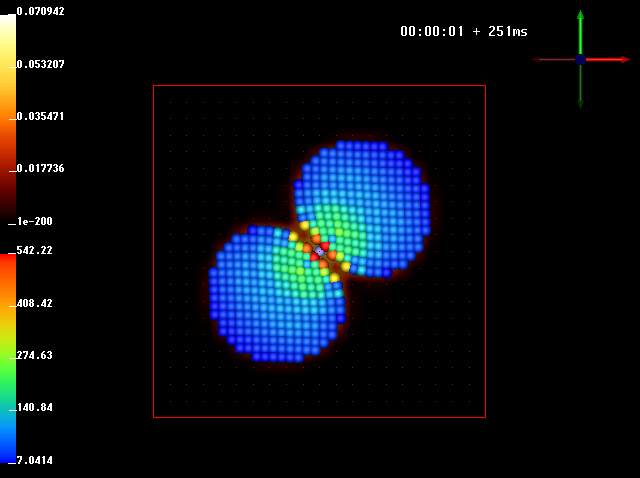
\includegraphics[width=0.5\textwidth]{disks.png}
  \caption{Colliding elastic disks.  Particles colored according to
velocity magnitude.}
  \label{figdisks}
\end{figure}

Additional data is available within the uda in the form of "dat" files.
In this case, both the kinetic and strain energies are avaiable and can
be plotted to create a graph similar to that in Fig. 5a of \cite{Sulsky1994}.
e.g. using gnuplot:

\begin{lstlisting}[backgroundcolor=\color{background}]
cd disks.uda.000
gnuplot
gnuplot> plot "StrainEnergy.dat", "KineticEnergy.dat"
gnuplot> quit
\end{lstlisting}
%
%__________________________________
\newpage
\subsection*{\center Taylor Impact Test}
\addcontentsline{toc}{subsection}{Taylor Impact Test}
\subsubsection*{\underline{Problem Description}}
This is a simulation of an Taylor impact experiment calculation from 
\cite{Gust1982} in a copper cylinder at 718 K that is fired at a
rigid anvil at 188 m/s.  The copper cylinder has a length of 30 mm and
a diameter of 6 mm.  The cylinder rebounds from the anvil after 100 $\mu$s.
 
\subsubsection*{\underline{Simulation Specifics}}
\begin{description} 
\item [Component used:] \hfill MPM
\item [Input file name:] \hfill taylorImpact.ups
\item [Command used to run input file:]\hfill vaango inputs/MPM/taylorImpact.ups
\item [Simulation Domain:]\hfill 8 mm x 33 mm x 8 mm

\item [Cell Spacing:]\hfill \\ 
  1/3 mm x 1/3 mm x 1/3 mm (Level 0)

\item [Example Runtimes:] \hfill \\
  1 hour   (1 processor, Xeon 3.16 GHz)\\

\item [Physical time simulated:] \hfill 100 $\mu$seconds

\item [Associate VisIt session:] \hfill taylorImpact.session

\end{description}

\subsubsection*{\underline{Results}}
Figure~\ref{fig:taylorImpact}(a) shows a snapshot from the end of the simulation.
There, the cylinder is allowed to slide laterally across the plate due
to the following optional specification in the \Textsfc{contact}
section:

\begin{lstlisting}[language=XML]
        <direction>[0,1,0]</direction>
\end{lstlisting}

\begin{figure}
  \centering
  \begin{subfigure}{0.4\textwidth}
    \centering
    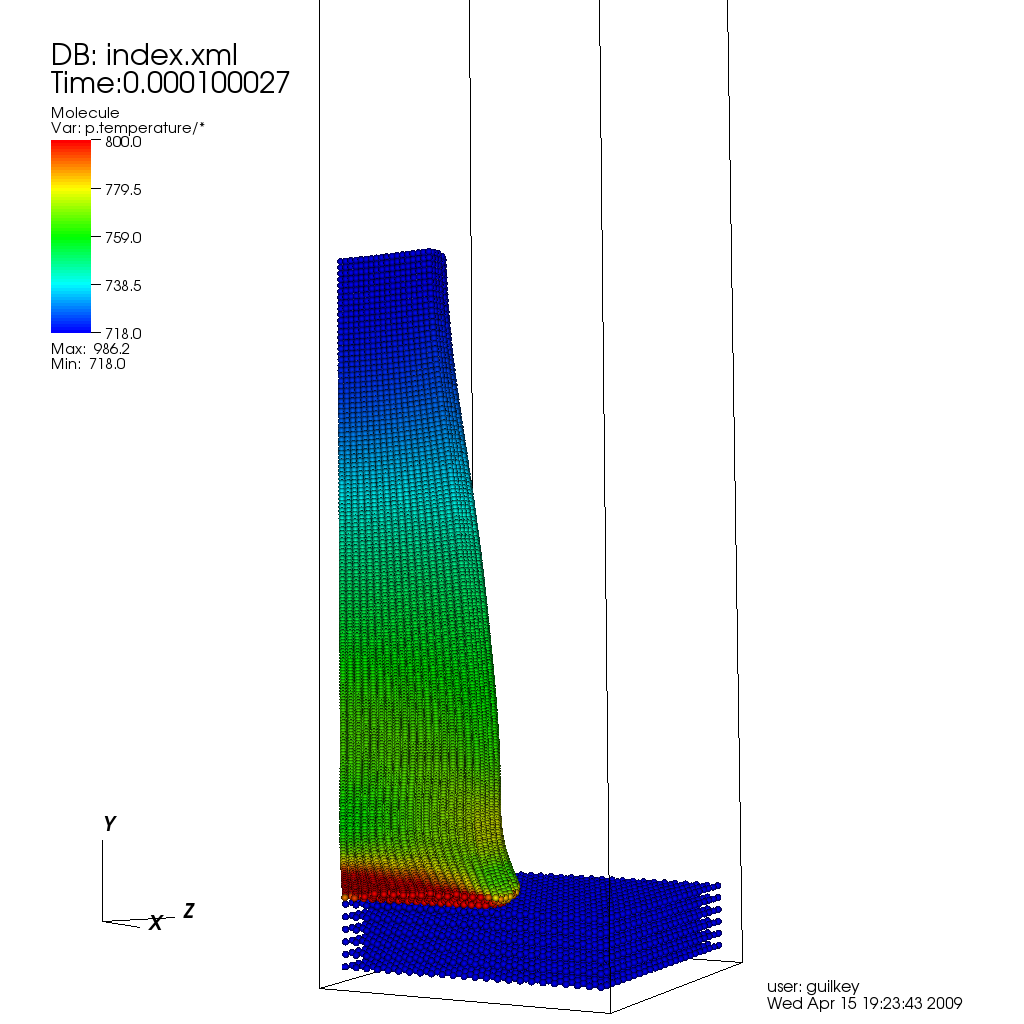
\includegraphics[height=0.3\textheight]{taylorImpact_slide.png}
    \label{fig:taylorImpact_slide}
    \caption{Sliding allowed}
  \end{subfigure}
  \begin{subfigure}{0.4\textwidth}
    \centering
    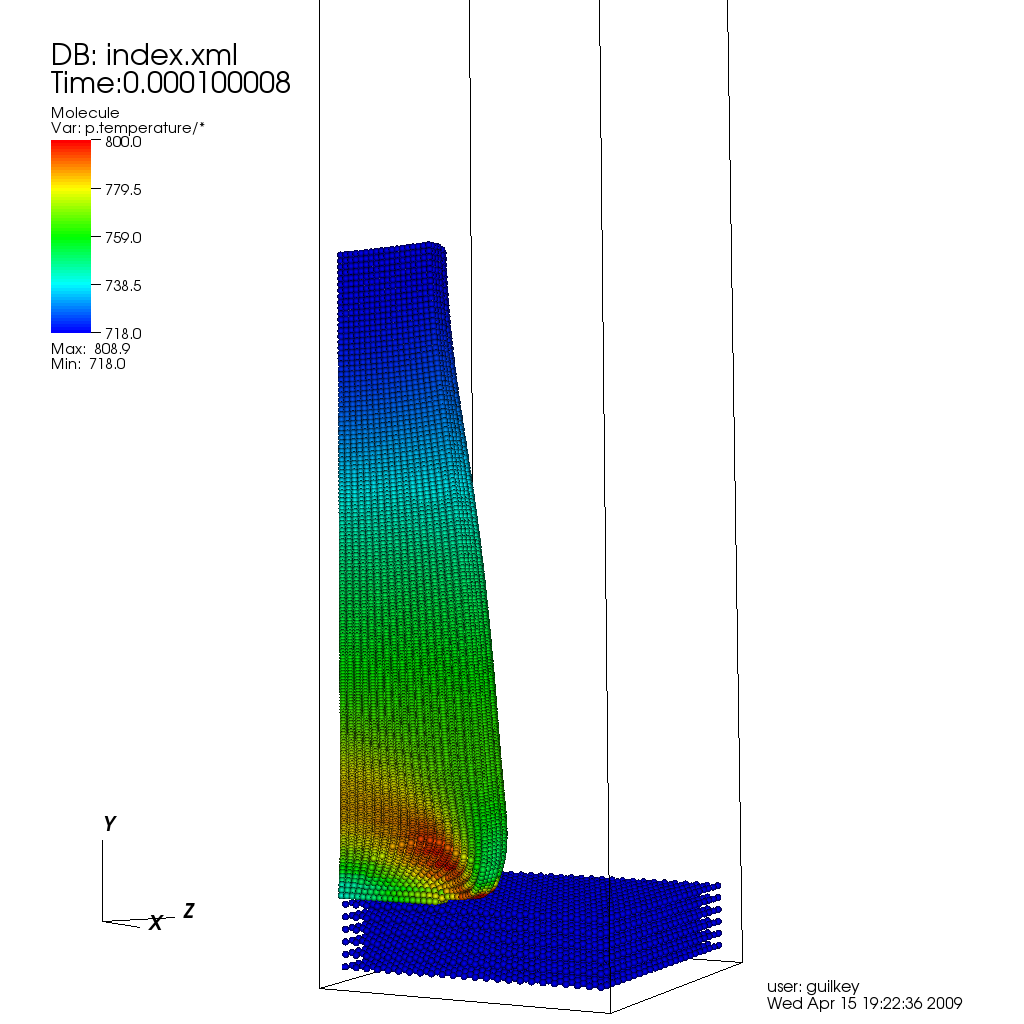
\includegraphics[height=0.3\textheight]{taylorImpact_stick.png}
    \label{fig:taylorImpact_stick}
    \caption{Sliding prohibited}
  \end{subfigure}
  \caption{Taylor impact simulation with (a) sliding (b) no sliding,
           between cylinder and
           target.  Particles colored according to temperature.}
  \label{fig:taylorImpact}
\end{figure}

Figure~\ref{fig:taylorImpact}(b) shows a snapshot from the end of a
similar simulation.  In this case, the cylinder is restricted from sliding
laterally across the plate by altering the \Textsfc{contact}
section as follows:
\begin{lstlisting}[language=XML]
        <direction>[1,1,1]</direction>
\end{lstlisting}

%__________________________________
\newpage
\subsection*{\center Sphere Rolling Down an Inclined Plane}
\addcontentsline{toc}{subsection}{Sphere Rolling Down an Inclined Plane}
\subsubsection*{\underline{Problem Description}}
Here, a sphere of soft plastic, initially at rest, rolls under the
influence of gravity down a plane of a harder plastic.  Gravity is
oriented such that the plane is effectively angled at 45 degrees to
the horizontal.  This simulation demonstrates the effectiveness of
the contact algorithm, described in~\cite{Bard2001}.  Frictional
contact, using a friction coefficient of $\mu = 0.495$ causes the ball
to start rolling as it impacts the plane, after being dropped from
barely above it.  The same simulation is also run using a friction
coefficient of $\mu = 0.0$.  The difference in the results is shown
below.
 
\subsubsection*{\underline{Simulation Specifics}}
\begin{description} 
\item [Component used:] \hfill MPM
\item [Input file name:] \hfill inclinedPlaneSphere.ups
\item [Command used to run input file:]\hfill vaango inputs/MPM/inclinedPlaneSphere.ups
\item [Simulation Domain:]\hfill    12.0 x 2.0 x 4.8 m

\item [Cell Spacing:]\hfill \\ 
.2 x .2 x .2 m (Level 0)

\item [Example Runtimes:] \hfill \\
 2.7 hours  (1 core, 3.16 GHz Xeon)\\

\item [Physical time simulated:] \hfill 2.2 seconds

\item [Associate VisIt session:] \hfill incplane.session

\end{description}

\subsubsection*{\underline{Results}}
Figure~\ref{figincplaneSphere}(a) and Figure~\ref{figincplaneSphere}(b)
show snapshots of the simulation, as
the sphere is about halfway down the plane.
\begin{figure}
  \centering
  \begin{subfigure}{0.4\textwidth}
    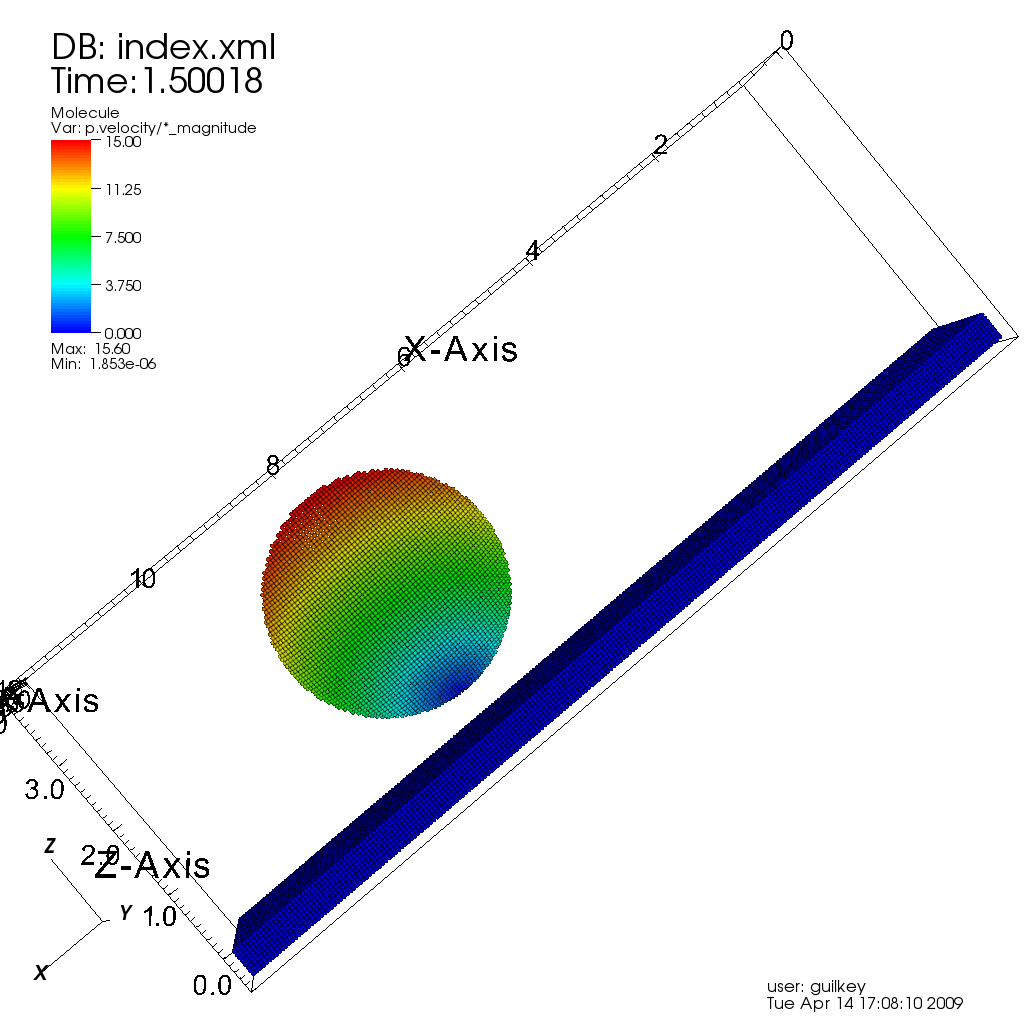
\includegraphics[width=\textwidth]{incplane_mu_495.png}
    \caption{Friction coefficient $\mu = 0.495$.}
    \label{figincplaneSphere_bigmu}
  \end{subfigure}
  \begin{subfigure}{0.4\textwidth}
    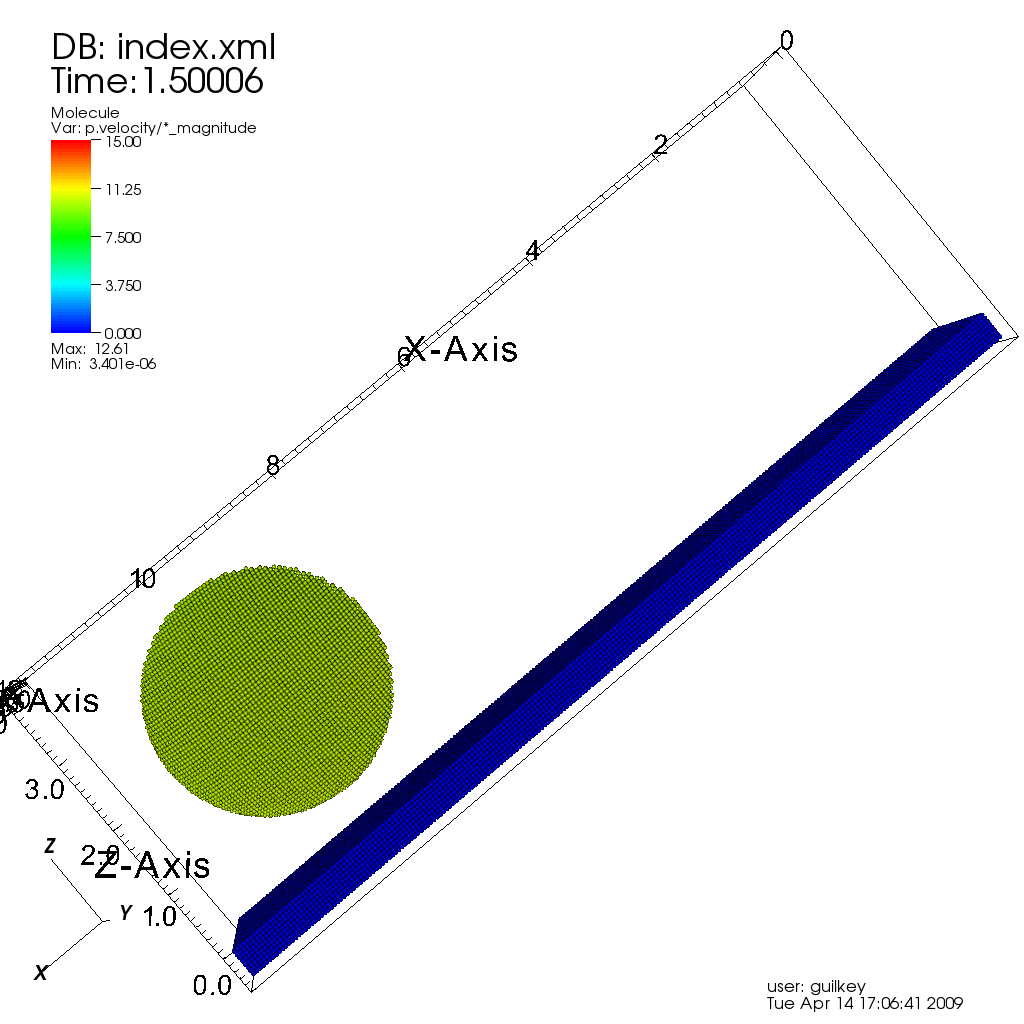
\includegraphics[width=\textwidth]{incplane_mu_0.png}
    \caption{Friction coefficient $\mu = 0$.}
    \label{figincplaneSphere_0mu}
  \end{subfigure}
  \caption{Sphere rolling down an ``inclined" plane.  The gravity vector
is oriented at a 45 degree angle relative to the plane.  Particles are colored
by velocity magnitude. 
Particles are colored according
to velocity magnitude, note that the particles at the top of the sphere
are moving most rapidly, and those near the surface of the plane are 
basically stationary, as expected.}
  \label{figincplaneSphere}
\end{figure}

%__________________________________
\newpage
\subsection*{\center Crushing a Foam Microstructure}
\addcontentsline{toc}{subsection}{Crushing a Foam Microstructure}
\subsubsection*{\underline{Problem Description}}
This calculation demonstrates two important strength of MPM.  The first
is the ability to quickly generate a computational representation of
complex geometries.  The second is the ability of the method to handle
large deformations, including self contact.

In particular, in this calculation a small sample of foam, the geometry
for which was collected using microCT, is represented via material points.
The sample is crushed to 87.5\% compaction through the use of a rigid plate, which
acts as a constant velocity boundary condition on the top of the sample.  This
calculation is a small example of those described in \cite{brydonfoam}.  The
geometry of the foam is created by image procesing the CT data, and based
on the intensity of each voxel in the image data, the space represented
by that voxel either recieves a particle with the material properties of the
foam's constituent material, or is left as void space.  This particle
representation avoids the time consuming steps required to build a suitable
unstructured mesh for this very complicated geometry.
 
\subsubsection*{\underline{Simulation Specifics}}
\begin{description} 
\item [Component used:] \hfill MPM
\item [Input file name:] \hfill foam.ups
\item [Instruction to run input file:]

First, copy foam.ups and foam.pts.gz to the same directory as \Textsfc{vaango}.
Adjust the number of patches in the ups file based on
the number of processors available to you for this run.
First, uncompress the pts file:
\begin{lstlisting}[backgroundcolor=\color{background}]
 gunzip foam.pts.gz
\end{lstlisting}

Then the command:
\begin{lstlisting}[backgroundcolor=\color{background}]
 tools/pfs/pfs foam.ups
\end{lstlisting}
will divide the foam.pts
file, which contains the geometric description of the foam,
into number of patches smaller files, named foam.pts.0,
foam.pts.1, etc.  This is done so that for large simulations,
each processor is only reading that data which it needs, and
prevents the thrashing of the file system that would occur
if each processor needed to read the entire pts file.  This
command only needs to be done once, or anytime the patch
distibution is changed.  Note that this step must be done even
if only one processor is available.

To run this simulation:
\begin{lstlisting}[backgroundcolor=\color{background}]
  mpirun -np NP vaango foam.ups
\end{lstlisting}
where NP is the number of processors being used.

\item [Simulation Domain:]\hfill  0.2 X 0.2 X 0.2125 mm

\item [Number of Computational Cells:]\hfill \\ 
102 X 102 X 85 (Level 0)

\item [Example Runtimes:] \hfill \\
2.4 hours  (4 cores, 3.16 GHz Xeon)\\

\item [Physical time simulated:] \hfill 3.75 seconds

\item [Associated VisIt session 1:] \hfill foam.iso.session
\item [Associated VisIt session 2:] \hfill foam.part.session

\end{description}

\subsubsection*{\underline{Results}}

Figure~\ref{figfoam_}(a) shows a snapshot of the simulation via isosurfacing,
as the foam is at about 50\% compaction.
\begin{figure}
  \centering
  \begin{subfigure}{0.4\textwidth}
    \centering
    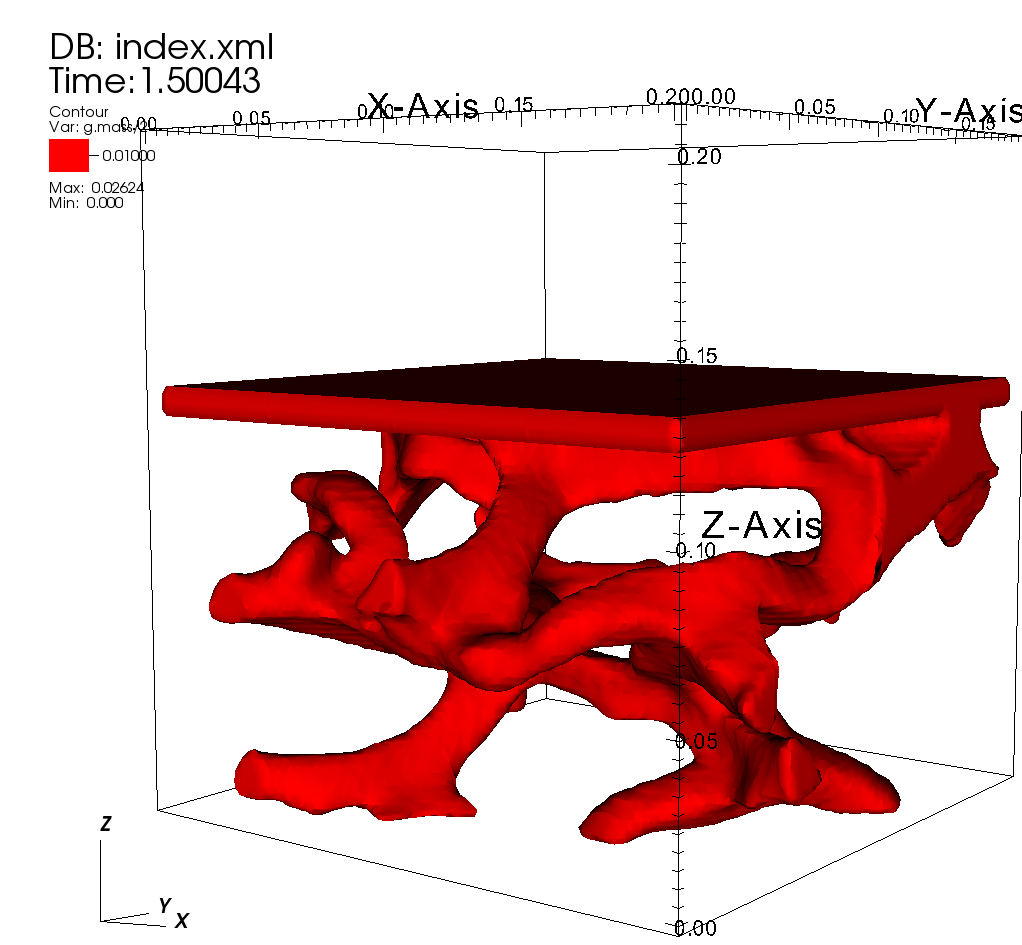
\includegraphics[width=\textwidth]{foam_iso.png}
    \caption{Rendered via isosurfacing.}
    \label{figfoam}
  \end{subfigure}
  \hspace{12pt}
  \begin{subfigure}{0.4\textwidth}
    \centering
    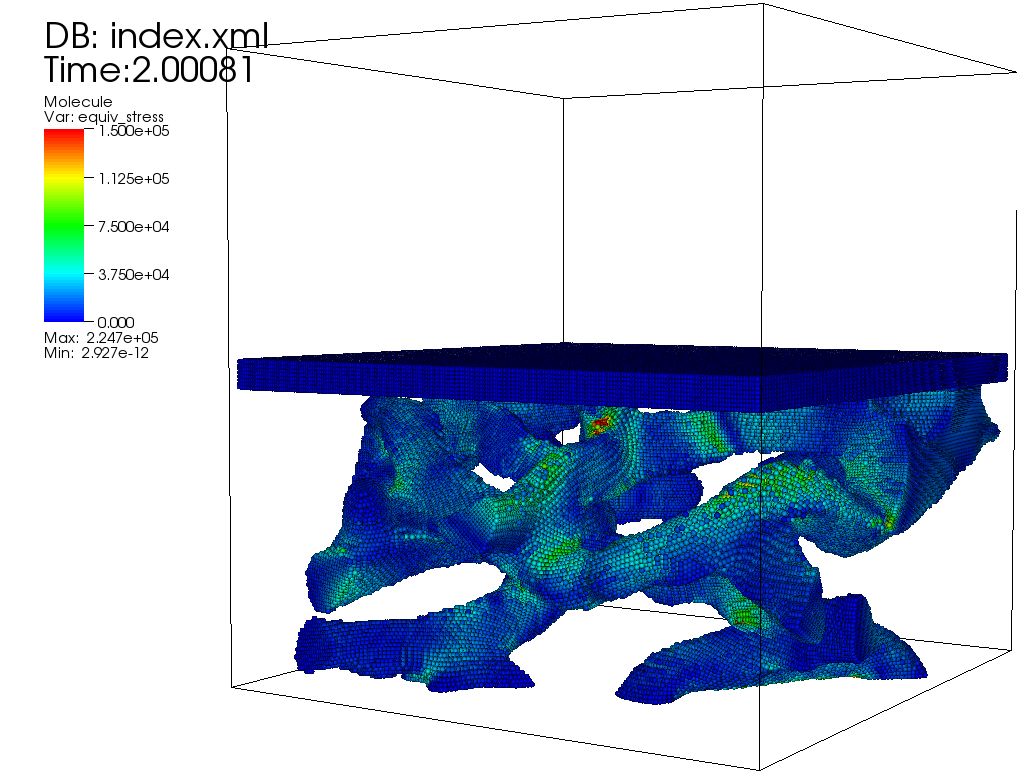
\includegraphics[width=\textwidth]{foam_part.png}
    \caption{Rendered with particles colored by equivalent stress.}
    \label{figfoampart}
  \end{subfigure}
  \caption{Compaction of a foam microstructure.}
  \label{figfoam_}
\end{figure}

Figure~\ref{figfoam_}(b) shows a snapshot of the simulation via particles
colored by equivalent stress as the foam is at about 60\% compaction.

In this simulation, the reaction forces at 5 of the 6 computational boundaries
are also recorded and can be viewed using a simple plotting package such
as gnuplot.  At each timestep, the internal force at each of the boundaries
is accumulated and stored in ``dat" files within the uda,
e.g. BndyForce\_zminus.dat.  Because the reaction force is a vector, it
is enclosed in square brackets which may be removed by use of a script in
the inputs directory:

\begin{lstlisting}[backgroundcolor=\color{background}]
cd foam.uda.000
../inputs/ICE/Scripts/removeBraces BndyForce\_zminus.dat
gnuplot
gnuplot> plot "BndyForce\_zminus.dat" using 1:4
gnuplot> quit
\end{lstlisting}

These reaction forces are similar to what would be measured on a mechanical
testing device, and help to understand the material behavior.

%__________________________________
\newpage
\subsection*{\center Hole in an Elastic Plate}
\addcontentsline{toc}{subsection}{Hole in an Elastic Plate}
\subsubsection*{\underline{Problem Description}}
A flat plate with a hole in the center is loaded in tension.  To achieve a
quasi-static solution, the load is applied slowly and a viscous damping force
is used to reduce transients in the solution.  As such, this simulation
demonstrates those two capabilities.  Specifically, take note of:
\begin{lstlisting}[language=XML]
       <use_load_curves> true </use_load_curves>
       <artificial_damping_coeff>1.0</artificial_damping_coeff>
\end{lstlisting}
in the \Textsfc{MPM} section of the input file, and:
\begin{lstlisting}[language=XML]
   <PhysicalBC>
     <MPM>
       <pressure>
  .
  .
  .
\end{lstlisting}
section below that.

 
\subsubsection*{\underline{Simulation Specifics}}
\begin{description} 
\item [Component used:] \hfill MPM
\item [Input file name:] \hfill holePlate.ups
\item [Command used to run input file:]\hfill vaango inputs/MPM/holePlate.ups
\item [Simulation Domain:]\hfill 5.0 m x 5.0 m x 0.1 m

\item [Cell Spacing:]\hfill \\ 
  0.1 m x 0.1 m x 0.1 m (Level 0)

\item [Example Runtimes:] \hfill \\
 2 minutes  (1 processor, Xeon 3.16 GHz)\\

\item [Physical time simulated:] \hfill 10 seconds

\item [Associate VisIt session:] \hfill holeInPlate.session

\end{description}

\subsubsection*{\underline{Results}}

Figure~\ref{fig:holeInPlate} shows a snapshot of the equivalent stress
throughout the plate, as well as the load applied to the vectors near the
edge of the plate.  Expected maximum stress is $300 Pa$.  The $238 Pa$ maximum
observed here is significantly lower, but upon doubling the resolution in the
x and y directions, the maximum stress is $308 Pa$.  To recreate this image, select
Controls in the upper left corner of the screen.  Select Expressions, then click the New 
button.  Now select Insert Function, then Tensor, then effective\_tensor.  The last step is
to select Insert Variable, then Tensor, then p. stress.  

\begin{figure}
  \center
  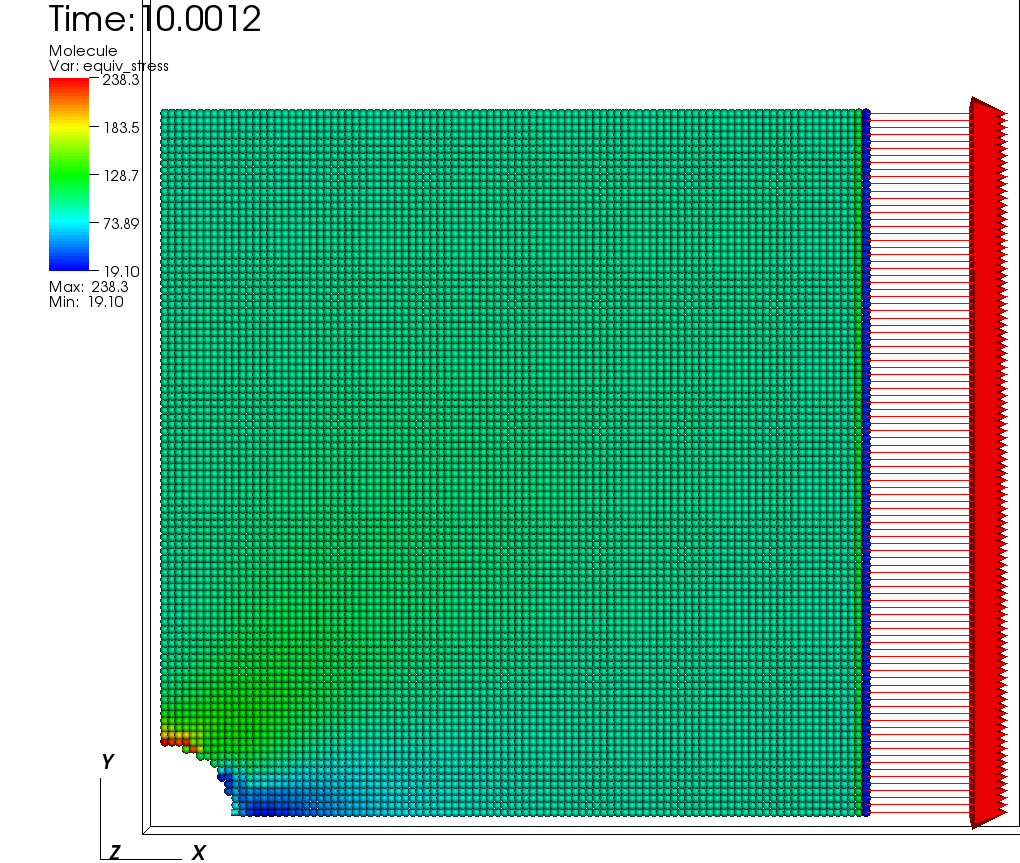
\includegraphics[width=0.5\textwidth]{holeInPlate.png}
  \caption{Elastic plate with a hole loaded in tension.  Particles are
           colored by equivalent stress, vectors indicate applied load.}
  \label{fig:holeInPlate}
\end{figure}

%__________________________________
\newpage
\subsection*{\center Tungsten Sphere Impacting a Steel Target}
\addcontentsline{toc}{subsection}{Tungsten Sphere Impacting a Steel Target}
\subsubsection*{\underline{Problem Description}}
A $1 mm$ tungsten sphere with an initial velocity of $5000 m/s$
impacts a steel target.  Axisymmetric conditions are used in this case,
conversion of the input file to the full 3D simulation is straightforward.
The user may wish to do both simulations of both to gain confidence in the
applicability of axisymmetry. 

This simulation exercises the \Textsfc{elastic\_plastic}
constitutive model for the
steel material. This includes sub-models for equations of state,
variable shear modulus, melting, plasticity, etc.  The tungsten is modeled
using the \Textsfc{comp\_neo\_hook\_plastic,} which is simple vonMises
plasticity with linear hardening.  One difficulty with using the more 
sophisticated models is that parameters can be difficult to find for many
materials.

\subsubsection*{\underline{Simulation Specifics}}
\begin{description}
\item [Component used:] \hfill MPM
\item [Input file name:] \hfill WSphereIntoSteel.axi.ups
\item [Command used to run input file:]\hfill vaango inputs/MPM/WSphereIntoSteel.axi.ups
\item [Simulation Domain:]\hfill 1.0 cm x 1.5 cm x axisymmetric

\item [Cell Spacing:]\hfill \\
  0.333 mm x 0.333 mm x axisymmetry (Level 0)

\item [Example Runtimes:] \hfill \\
 15 seconds  (1 processor, Xeon 3.16 GHz)\\

\item [Physical time simulated:] \hfill 4 $\mu$seconds

\item [Associate VisIt session:] \hfill WSphereSteel.session

\end{description}

\subsubsection*{\underline{Results}}

Figure~\ref{fig:WSphereSteelInit} shows the initial configuration for
this simulation, with particles colored by the magnitude of their velocity.
Figure~\ref{fig:WSphereSteelFinal} shows the state of the simulation after
$4 \mu$seconds this simulation, with particles still colored by velocity
magnitude.

\begin{figure}
  \center
  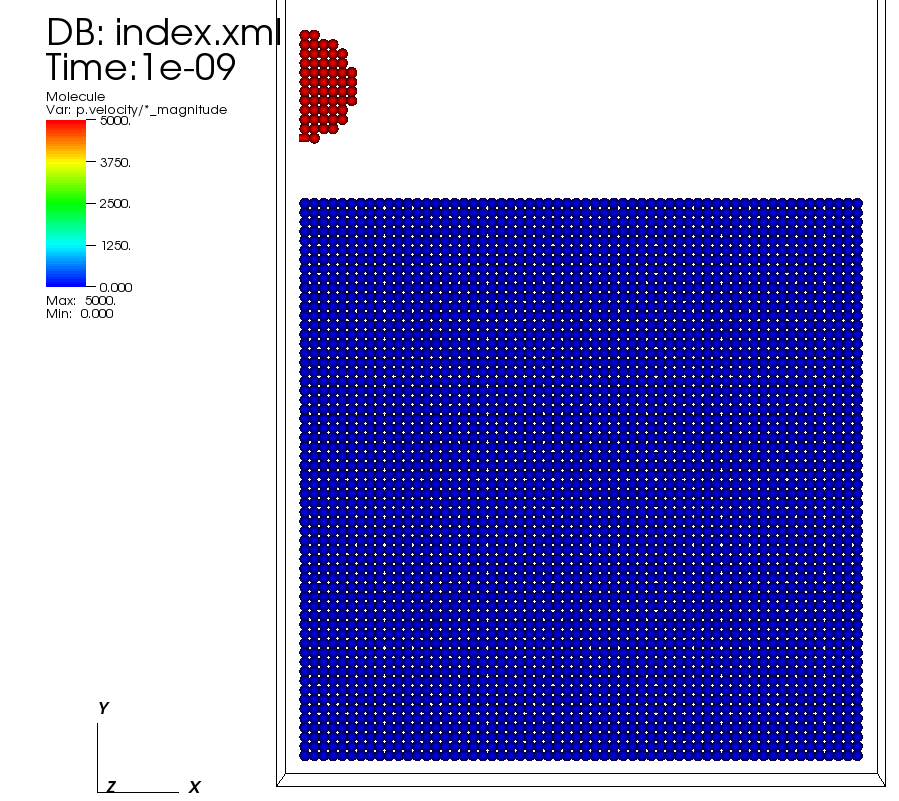
\includegraphics[width=0.5\textwidth]{WShereInitAxi.png}
  \caption{Initial configuration of hypervelocity impact of tungsten sphere
           into a steel target.  Particles are
           colored by velocity magnitude.}
  \label{fig:WSphereSteelInit}
\end{figure}
\begin{figure}
  \center
  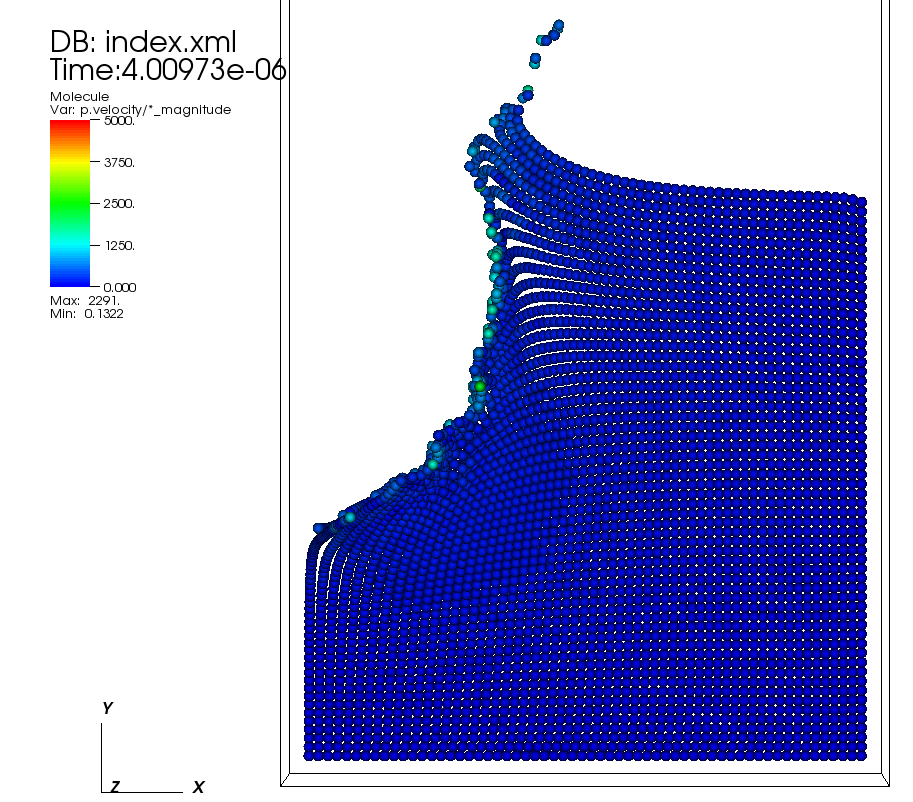
\includegraphics[width=0.5\textwidth]{WShereFinalAxi.png}
  \caption{State of the tunsgsten and steel after $4 \mu$seconds.
           Particles are colored by velocity magnitude.}
  \label{fig:WSphereSteelFinal}
\end{figure}

\newpage
\section{Method Of Manufactured Solutions (MMS)}
There are three manufactured solutions available in \Vaango for nonlinear elastic constitutive models. The input files are available in the \Textsfc{inputs/MPM} folder. 
\begin{lstlisting}[backgroundcolor=\color{background}]
AA.ups (Axis Aligned MMS)
GenVortex.ups (Genralized Vortex MMS)
Ring_MMS.ups (Expanding Ring MMS)
\end{lstlisting}
All these input files have the following tag included in the \Textsfc{MPM} section of the input file:
\begin{lstlisting}[language=XML]
<MPM>
   <RunMMSProblem>Name of the MMS</RunMMSProblem>  
</MPM>
\end{lstlisting}
The exact solutions for these problems are available in \Textsfc{puda}, and the call to extract the error is
\begin{lstlisting}[backgroundcolor=\color{background}]
puda -AA_MMS_2 AA_MMS.uda (for AxisAligned MMS)
puda -GV_MMS GenVortex.uda (for Generalized Vortex MMS)
puda -ER_MMS Ring_MMS.uda (for Expanding Ring MMS)
\end{lstlisting}

The current implementation allows the user to add a new manufactured solution in the \Textsfc{MPM} component in a relatively-straight forward way. The current implementation of these manufactured solutions are located in \Textsfc{src/CCA/Components/MPM/MMS} folder.
The following files require modifications either to change the exisiting MMS or add a new one.
\begin{lstlisting}[backgroundcolor=\color{background}]
1) src/CCA/Components/MPM/MPMFlags.cc
2) src/StandAlone/inputs/UPS_SPEC/mpm_spec.xml
3) src/CCA/Components/MPM/MMS/MMS.cc
4) src/CCA/Components/MPM/ConstitutiveModel/CNH_MMS.cc (Right now, all these MMS use
the same constitutive model. User can change the constitutive model accordingly)
5) src/StandAlone/tools/puda/puda.cc
\end{lstlisting}
Following are the sequential steps to add a new MMS to the existing framework. 
\newline
1) In \Textsfc{MPMFlags.cc}, add another \Textsfc{if} condition for the new MMS string in the following \Textsfc{loop}
\begin{lstlisting}[language=Cpp]
if(d_mms_type=="AxisAligned"){
    d_mms_type = "AxisAligned";
  } else if(d_mms_type=="GeneralizedVortex"){
    d_mms_type = "GeneralizedVortex";
  } else if(d_mms_type=="ExpandingRing"){
    d_mms_type = "ExpandingRing";
  } else if(d_mms_type=="AxisAligned3L"){
    d_mms_type = "AxisAligned3L";
  }
}
\end{lstlisting}
2) Add the same string in the \Textsfc{RunMMSProblem} tag located in the \Textsfc{mpm\_spec.xml} file.
\newline
3) There are two member functions available in \Textsfc{MMS.cc}.
\begin{lstlisting}[language=Cpp]
    MMS::initializeParticleForMMS
    MMS::computeExternalForceForMMS
\end{lstlisting}
Similar to step $1$, add another \Textsfc{if} condition in both the member functions for the new MMS. In the \Textsfc{initializeParticleForMMS} function, initialize the particle data at time $t=0$, and in the \Textsfc{computeExternalForceForMMS} function, code the analytical body forces. The exisiting analytical solutions can be used as a guide.
\newline
4) Add the exact solution in the \Textsfc{src/StandAlone/tools/puda} folder. Look at the \Textsfc{AA\_MMS.cc, GV\_MMS.cc, and ER\_MMS.cc} for reference. Add the option for the new MMS in the \Textsfc{puda.cc} file.
\newline
5) If the new MMS has a non-zero stress, necessary modifications needs to be made in the \Textsfc{initializeCMData} function located in that particular constitutive model (CNH\_MMS.cc for reference).

